
\documentclass[11pt,a4paper]{report}
% sostituire con report/book per il formato elettronico

\usepackage[nottoc,notlof,notbib,notindex]{tocbibind} % include l'elenco delle figure e la bibliografia nell'indice.

\usepackage{appendix}
\usepackage{array}
\usepackage{multirow}
\usepackage[english]{babel}
\usepackage{ucs} %unicode sistema gli accenti
\usepackage[utf8x]{inputenc} %unicode sistema gli accenti utf8x
\usepackage[bottom]{footmisc} % posiziona le note in footer sempre in basso
\usepackage{fancyhdr}
\usepackage{graphicx}
\usepackage{color}
\usepackage{subfigure} % per figure affiancate
\usepackage{supertabular} % used to break tables
\usepackage{float} % per far bene le figures
%\usepackage{indentfirst}
\usepackage[Lenny]{fncychap} % per cambiare i capitoli
\usepackage{longtable} % piazza le note nelle tabelle fuori dalla tabella e permette tabelle che spannano su più pagine
\usepackage{lastpage} % total page count
\usepackage[hyphens]{url}
%\usepackage{breakurl}
\usepackage{amsmath}
\usepackage{amssymb}
\usepackage{comment}
\usepackage{amsthm}
\usepackage{url}
\usepackage{amsmath}
\usepackage[table]{xcolor} % For coloring cells
\usepackage[colorlinks=true, pdfstartview=FitV, linkcolor=blue, citecolor=blue, urlcolor=blue,breaklinks=true]{hyperref}

% To be able to use argmax
\DeclareMathOperator*{\argmin}{arg\,min}

% colori e variabili
% color definitions
\definecolor{red}{rgb}{0.9,0.1,0.1}
\definecolor{blue}{rgb}{0.07,0.55,0.73}
\definecolor{purple}{rgb}{0.4,0.3,0.4}
\definecolor{deep}{rgb}{0.1,0.07,0.3}
\definecolor{white}{rgb}{0.9,0.8,0.86}
% per modificare il colore dei link andare su layout.tex
%layout legacy commands
\renewcommand{\sectionmark}[1]{\markright{\thesection.\ #1}}
\renewcommand{\chaptermark}[1]{\markboth{\thechapter.\ #1}{}}

%user defined commands

% defnisce una pagina bianca con stile plain (migliore delle pagine bianche inserite in automatico dal model book)
\newcommand{\blankpage}{
	\newpage
	% toglie la barra alta dalla pagina vuota
	\thispagestyle{plain}
	% forza una pagina vuota
	\mbox{}
	\newpage
}

%comando per inserire la premessa nel documento (fuori indice)
\newcommand{\premise}[1][]{
	\renewcommand{\theenumi}{#1\roman{enumi}}
	\renewcommand{\labelenumi}{(\theenumi)}
	\thispagestyle{plain}
}


%comandi creati per le convenzioni del documento:
\newcommand{\istage}{\textit{stage}}
\newcommand{\iStage}{\textit{Stage}}
\newcommand{\idfda}{\textit{D.F.D. Assessment System}}
\newcommand{\idfd}{\textit{D.F.D. Consulting}}
\newcommand{\iIT}{\textit{IT}}
\newcommand{\iICT}{\textit{ICT}}
\newcommand{\ibusiness}{\textit{business}}





% indice analitico (comandi con la 'i' scrivono e aggiungono, quelli con 'ii' aggiungono solo, quelli senza niente scrivono solo)
\newcommand{\iASI}{ASI\index{ASI}} %scrive C sharp

%tecnologie
\newcommand{\CSharp}{C♯} %scrive C sharp
\newcommand{\iCSharp}{C♯\index{C♯}} % scrive C sharp e aggiunge l'indice %\unichar{9839}
\newcommand{\idotNET}{.NET\index{.NET}} % scrive .NEt e aggiunge l'indice
\newcommand{\iiWPF}{\index{WPF}} % aggiunge solo l'indice a WPF
\newcommand{\iWPF}{WPF\index{WPF}} % scrive WPF e aggiunge l'indice
\newcommand{\iiWF}{\index{WinForms}}
\newcommand{\iAW}{ANTLRWorks\index{ANTLRWorks}}
\newcommand{\iA}{ANTLR\index{ANTLR}}
\newcommand{\iU}{Unicode\index{Unicode}}
\newcommand{\iPSharp}{\texttt{PdfSharp}\index{PdfSharp@\texttt{PdfSharp}}}
\newcommand{\iTSharp}{\texttt{iTextSharp}\index{iTextSharp@\texttt{iTextSharp}}}

%grammatica
\newcommand{\iiCFG}{\index{CFG (context-free grammar)}}

%programmi
\newcommand{\iVS}{Visual Studio\index{Visual Studio}}
\newcommand{\iVSS}{Visual SourceSafe\index{Visual SourceSafe}}
\newcommand{\iSS}{SQL Server\index{SQL Server}}

% ciclo attivo e passivo
\newcommand{\iCA}{ciclo attivo\index{ciclo!attivo}} % scrive ciclo attivo e aggiunge l'indice
\newcommand{\iCP}{ciclo passivo\index{ciclo!passivo}} % scrive ciclo passivo e aggiunge l'indice
\newcommand{\iiCA}{\index{ciclo!attivo}} % aggiunge l'indice
\newcommand{\iiCP}{\index{ciclo!passivo}} % aggiunge l'indice
\newcommand{\iDCA}{ciclo attivo\index{documento!ciclo attivo}} % scrive ciclo attivo agigunge l'indice al ciclo attivo del documento
\newcommand{\iDCP}{ciclo passivo\index{documento!ciclo passivo}} % scrive ciclo passivo aggiunge l'indice al ciclo passivo del documento
\newcommand{\iiDCA}{\index{documento!ciclo attivo}} % aggiunge l'indice al ciclo attivo del documento
\newcommand{\iiDCP}{\index{documento!ciclo passivo}} % aggiunge l'indice al ciclo passivo del documento
\newcommand{\iGCA}{ciclo attivo\index{gestione!ciclo attivo}} % scrive ciclo attivo e aggiunge l'indice a gestione
\newcommand{\iGCP}{ciclo passivo\index{gestione!ciclo passivo}} % scrive ciclo passivo e aggiunge l'indice a gestione
\newcommand{\iiGCP}{\index{gestione!ciclo passivo}} % aggiunge l'indice a gestione

%componenti
\newcommand{\icMM}{\texttt{MapManager}\index{MapManager@\texttt{MapManager}}}
\newcommand{\iicMM}{\index{MapManager@\texttt{MapManager}}}
\newcommand{\icMF}{\texttt{MapFinder}\index{MapFinder@\texttt{MapFinder}}}
\newcommand{\iicMF}{\index{MapFinder@\texttt{MapFinder}}}
\newcommand{\icPA}{\texttt{PdfAnalyzer}\index{PdfAnalyzer (componente)@\texttt{PdfAnalyzer} (componente)}}

%package e classi
\newcommand{\iPFE}{\texttt{Plain.File.Extraction}\index{Plain.File.Extraction@\texttt{Plain.File.Extraction}}}
\newcommand{\iiPFE}{\index{Plain.File.Extraction@\texttt{Plain.File.Extraction}}}
\newcommand{\iPA}{\texttt{PdfAnalyzer}\index{Plain.File.Extraction@\texttt{Plain.File.Extraction}!PdfAnalyzer (classe)@\texttt{PdfAnalyzer} (classe)}}
\newcommand{\iPP}{\texttt{PdfPage}\index{Plain.File.Extraction@\texttt{Plain.File.Extraction}!PdfPage@\texttt{PdfPage}}}
\newcommand{\iPPar}{\texttt{PdfTextStreamParser}\index{Plain.File.Extraction@\texttt{Plain.File.Extraction}!PdfTextStreamParser@\texttt{PdfTextStreamParser}}}
\newcommand{\iPLex}{\texttt{PdfTextStreamLexer}\index{Plain.File.Extraction@\texttt{Plain.File.Extraction}!PdfTextStreamLexer@\texttt{PdfTextStreamLexer}}}
\newcommand{\iPF}{\texttt{PdfFont}\index{Plain.File.Extraction@\texttt{Plain.File.Extraction}!PdfFont@\texttt{PdfFont}}}
\newcommand{\iPT}{\texttt{PdfText}\index{Plain.File.Extraction@\texttt{Plain.File.Extraction}!PdfText@\texttt{PdfText}}}
\newcommand{\iPC}{\texttt{PdfChar}\index{Plain.File.Extraction@\texttt{Plain.File.Extraction}!PdfChar@\texttt{PdfChar}}}

%parti di un PDF
\newcommand{\iH}{\texttt{Header}\index{PDF!Header@\texttt{Header}}}
\newcommand{\iFT}{\texttt{File Trailer}\index{PDF!File Trailer@\texttt{File Trailer}}}
\newcommand{\iCRTable}{\texttt{Cross Reference Table}\index{PDF!Cross Reference Table@\texttt{Cross Reference Table}}}
\newcommand{\iB}{\texttt{Body}\index{PDF!Body@\texttt{Body}}}

% stream
\newcommand{\iS}{stream\index{stream}}
\newcommand{\iiS}{\index{stream}}
\newcommand{\iCS}{stream\index{content stream}}
\newcommand{\iiCS}{\index{content stream}}

%fasi dello stage
\newcommand{\iifS}{\index{studio del dominio!fase di}}
\newcommand{\iifA}{\index{analisi!fase di}}
\newcommand{\iifP}{\index{progettazione!fase di}}
\newcommand{\iifC}{\index{codifica!fase di}}
\newcommand{\iifV}{\index{verifica e validazione!fase di}}
\newcommand{\iifD}{\index{documentazione!fase di}}

%attività dello stage
\newcommand{\iiaS}{\index{studio del dominio!attività di}}
\newcommand{\iiaA}{\index{analisi!attività di}}
\newcommand{\iiaP}{\index{progettazione!attività di}}
\newcommand{\iiaC}{\index{codifica!attività di}}
\newcommand{\iiaV}{\index{verifica e validazione!attività di}}
\newcommand{\iiaD}{\index{documentazione!attività di}}

%matrici
\newcommand{\Tm}{$T_{m}$}
\newcommand{\Tlm}{$T_{lm}$}

%peratori
\newcommand{\Tc}{\texttt{Tc}\index{operatore!di stato}}
\newcommand{\Tw}{\texttt{Tw}\index{operatore!di stato}}
\newcommand{\Tz}{\texttt{Tz}\index{operatore!di stato}}
\newcommand{\TL}{\texttt{TL}\index{operatore!di stato}}
\newcommand{\Tf}{\texttt{Tf}\index{operatore!di stato}}
\newcommand{\Tr}{\texttt{Tr}\index{operatore!di stato}}
\newcommand{\Ts}{\texttt{Ts}\index{operatore!di stato}}

\newcommand{\Td}{\texttt{Td}\index{operatore!di posizionamento}}
\newcommand{\Tmm}{\texttt{Tm}\index{operatore!di posizionamento}}
\newcommand{\Tstar}{\texttt{T*}\index{operatore!di posizionamento}}

\newcommand{\Tj}{\texttt{Tj}\index{operatore!di stampa}}
\newcommand{\Tquote}{\texttt{'}\index{operatore!di stampa}}
\newcommand{\Tdblquote}{\texttt{\textquotedbl}\index{operatore!di stampa}}
\newcommand{\TJ}{\texttt{TJ}\index{operatore!di stampa}}











\graphicspath{{./pics/}} % cartella di salvataggio immagini

\pagestyle{fancy}

\lhead{\nouppercase{\rightmark}}
\rhead{\nouppercase{\leftmark}}

\fancypagestyle{plain}{
	\lhead{}
	\chead{}
	\rhead{}
	\lfoot{}
	\cfoot{\thepage}
	\rfoot{}
	\renewcommand{\headrulewidth}{0.0pt}% this command should not be add to variables.tex
	\renewcommand{\footrulewidth}{0.1pt}% this command should not be add to variables.tex
}

\fancypagestyle{blank}{
	\lhead{}
	\chead{}
	\rhead{\nouppercase{\rightmark}}
	\lfoot{}
	\cfoot{\thepage}
	\rfoot{}
	\renewcommand{\headrulewidth}{0.1pt}% this command should not be add to variables.tex
	\renewcommand{\footrulewidth}{0.1pt}% this command should not be add to variables.tex
}



% parte per il report
 %	\lhead{}
% 	\chead{}
% 	\rhead{\nouppercase{\rightmark}}
% 	\lfoot{}
% 	\cfoot{\thepage}
% 	\rfoot{}
% 	\renewcommand{\headrulewidth}{0.1pt}% this command should not be add to variables.tex
% 	\renewcommand{\footrulewidth}{0.1pt}% this command should not be add to variables.tex
 
 %\hypersetup{
 %	colorlinks=true,% false: boxed links; true: colored links
% 	linkcolor=blue,% color of internal links
% 	urlcolor=blue,% color of external links
% 	anchorcolor = blue,
% 	citecolor = blue
 %}
%parte per il report



% parte per il book
\fancyhead{}
%\fancyhead[EL]{\nouppercase{\leftmark}}
\fancyhead[OR]{\nouppercase{\rightmark}}
%\fancyfoot[EC,OC]{\thepage}

	\renewcommand{\headrulewidth}{0.1pt}% this command should not be add to variables.tex
	\renewcommand{\footrulewidth}{0.1pt}% this command should not be add to variables.tex
\hypersetup{
	colorlinks=true,% false: boxed links; true: colored links
	linkcolor=black,% color of internal links
	urlcolor=black,% color of external links
	anchorcolor = black,
	citecolor = black
}
%parte per il book

% indice analitico
\usepackage{makeidx}
\makeindex 

\let\textquotedbl=" % use to print also " in the code

\bibliographystyle{plain}%bibliografia stile inglese

\pagenumbering{Roman}
% fine layout
% layout
\begin{document}

\hyphenation{
Kennt-nis-se An-wen-dungs-ge-bietes fle-xi-blen Emp-feh-lung-en
}


%word division
% Frontespizio
\begin{titlepage}
\begin{center}
	\vspace{6em}
	{\huge \textsc{Master Thesis}}\\
	\vspace{3em}
	{\huge \textsc{How Genomes are Shaped by Direct and Indirect Selection Pressure: A Study in in silico Experimental Evolution}}\\
	\vspace{3em}
	{\Large \textsc{Brian Davis}}\\
	\vspace{2em}
	{\Large \textsc{Supervisor: Berenice Batut}}\\
	\vspace{3em}
	{\Large \textsc{April 2020}}\\
	\vspace{5em}
	
\includegraphics[scale=1]{unifr-logo.jpg}\\
	\vspace{3em}
	{\Large \textsc{Albert-Ludwigs Universität Freiburg}}\\
	\vspace{2em}
	{\Large \textsc{Bioinformatics Group}}\\
	\vspace{2em}
	{\Large \textsc{Professor Dr. Rolf Backofen}}\\
\end{center}
\end{titlepage}%for the cover title

%If want to write a dedication, modify the following.
%\dedication{Zitat, kluger Spruch oder Widmung}

%
\newpage
%\pagestyle{empty}

\chapter*{Abstract}
\addcontentsline{toc}{chapter}{Abstract}
Not all aspects of evolution are fully understood, and one area of pressing interest is reductive evolution, in which the genome of a species evolves to become significantly smaller over time. Among the more well-known examples of this phenomena is \textit{Prochlorococcus}, a marine cyanobacteria whose genome has reduced up to 43\% among some of its own ecotypes and around 36\% smaller than some strains of its closest living relative, \textit{Synechococcus}. To study the mechanisms behind reductive evolution in the lab would be too difficult, expensive, and above all, slow, so instead \textit{in silico} evolution may be used to study this phenomenon. This method seeks to simulate organisms and their evolution in software, allowing for greater control of the environment, mutation rates, and other variables, as well as providing a full phylogenetic record of all organisms in a lineage. In this thesis the in silico tool Aevol is used to study reductive evolution, particularly by looking at how varying parameters (e.g. mutation and selection rates, population size) impacts the structure of the genome as well as measures such as robustness, evolvability, and fitness. Through these methods, a little light is shed on some of the underlying mechanisms which might lead to reductive evolution. 
%TODO Add summmry of results to abstract



% Old Abstract
%\newpage
%\blankpage
%\premise{
%\noindent{\textbf{\begin{huge}Abstract\end{huge}}}\\
%\\
%Abstract 
%}
\linespread{1.25}\selectfont

\tableofcontents
\addcontentsline{toc}{chapter}{\listfigurename}
\listoffigures  
\listoftables
\blankpage
\pagenumbering{arabic}%DO NOT REMOVE THIS
\chapter{Introduction}\label{ch:01intro}

One way of thinking about evolution is with regard to the change in frequencies of alleles (variants of genes) in a population over time. In the field of population genetics, the \textit{Hardy-Weinberg principle} states that genetic variation (diversity of gene frequencies) in a population will remain constant from generation to generation in the absence of disturbances \cite{cutter2019primer}. There are five ``Hardy-Weinberg assumptions'' which must hold for this to be true: no mutation, random mating, no gene flow (i.e. no transferring of genetic material from one population to another), infinite population sizes, and no selection. If any of these assumptions does not hold, then this may change the frequencies of alleles in a population, which allows evolution to occur. The mechanisms for evolution, then, are the opposite of these assumptions, namely: mutation, non-random mating, gene flow, finite populations, and natural selection. Pulling at any of these levers has an effect on the genetic variation of a population and thus impacts their genome. 

Several models have been proposed to illustrate the effects on the population of violating these assumptions. The \textit{Moran model}, named after the Australian statistician Patrick Moran, can be used on populations of finite size to model the impact of neutral drift (a mutation spreading through the population which has no impact on fitness), selection, or mutations. In the simplest version of the neutral drift model, for example, a population consists of two types, A and B, and in each generation one individual is randomly chosen to reproduce and another individual is randomly chosen to die. Given a population with $N$ individuals and $i$ individuals of one type ($0 \leq i \leq N$), the transition probabilities from one state to the next (increasing, decreasing, or maintaining the number of one type) can easily be calculated. The model concludes that given enough time, however, the population reaches \textit{``absorbing''} states in which the population is all of one type, either A or B, with a probability of $\frac{i}{N}$ due to all organisms having equal fitness (and thus being equally likely to be selected at random). The impact of genetic drift on bacterial genome size has been investigated extensively by Kuo et al.~\cite{kuo2009consequences} who found further evidence that ``evolutionary forces that act on individual genes have profound effects on the overall architecture of bacterial genomes.'' 

As mentioned above, changes to the population size also causes evolution to occur. The American geneticist Michael Lynch argued in a seminal paper, ``The Origins of Genome Complexity,'' that it was largely due to the increase in organism size\textemdash and thus the decrease in effective population size\textemdash that genome complexity increased, both in prokaryotes (e.g. bacteria) and eukaryotes (e.g. humans). This resulted in an increase in the number of genes and the amount of non-coding DNA, which in turn provided a basis for increased complexity. He argues: ``the transitions from prokaryotes to unicellular eukaryotes to multicellular eukaryotes are associated with orders-of-magnitude reductions in population size; by magnifying the power of random genetic drift, reduced population size provides a permissive environment for the proliferation of various genomic features that would otherwise be eliminated by purifying selection''~\cite{Lynch1401}. 

By contrast, reductive evolution is the process of the average genome size of a species shrinking over time, with respect to both the number of base pairs and genes. Reductive evolution is an interesting phenomenon because it was sometimes hypothesized that increasing genome size and genomic complexity (measured, for example, via the number of genes) were closely tied to the complexity of organisms. With the advent of genomic sequencing, however, it quickly became apparent that genome size (sometimes called the ``C-value'') and organismal complexity are not necessarily synchronized; this is known as the ``C-value paradox.'' 

As an example of reductive evolution, some species of bacteria have experienced reductive evolution over the course of millions of years, and this reduction in their genome has lead to a loss of genes, certain regulatory abilities, and more. It has also been theorized that reductive evolution may be responsible for the origin of eukaryotic cells, with the ``symbiogenesis'' theory suggesting that prokaryotic cells may have eventually become the organelles inside eukaryotic cells, with many of the prokaryotic genes being lost due to the mutualistic nature of living in the more protected environment of the cell body~\cite{sagan1967origin}. One free-living bacterial species which has exhibited clear tendencies towards reductive evolution is the marine cyanobacteria \textit{Prochlorococcus}, some of whose strains have experienced a reduction of nearly 40\% of their base pairs when compared to larger strains of their closest living relative,~\textit{Synechococcus}. Even among strains of Prochlorococcus, the difference between some of the larger and smaller strains is upwards of 38\%~\cite{Batut.2014}. Despite being extensively studied, the underlying mechanisms and full impact of reductive evolution are not fully understood and are an area of intense current research. Several competing explanations exist for these mechanisms, from the influence of population size, genetic drift (defined below), or selection~\cite{Batut.2014}, which are discussed in Chapter~\ref{ch:02background}. 

Previously, reductive evolution has also been studied via the methodology of comparative genomics, in which genomic features (e.g. DNA sequences, genes, gene order, etc.) were compared between organisms or species. The idea is that related organisms will have features in common which are encoded in their respective genomes, and that these features will have been conserved over the course of evolution. Often, an ``alignment'' of genomic sequences from two or more organisms is performed, in which the sequences are lined up so that matching positions in the sequence are correlated with each other, allowing one to see ``orthologous'' sequences (i.e. sequences of common ancestry). Based on these connections, evolutionary connections are inferred, based on the assumption that more closely-related genomes are more likely to be of recent common ancestry. This allows one to deduce phylogeny (evolutionary history and relatedness) of different organisms. In addition to the computational challenges presented by this approach, one of the biggest drawbacks of this methodology is that the individual steps are not easily identifiable; one may only analyze discreet moments in time (for which one has sequences), and any intermediate steps are lost to evolutionary time.  

Although it would provide more conclusive evidence, performing \textit{in vivo} experiments with living organisms is often impractical because of the difficulty or impossibility of reproducing natural environmental conditions in a laboratory. Such experiments are often too costly in terms of both time and resources. As an alternative, \textit{in silico} experimental evolution is one option that can be used to study the conditions under which an organism's genome may become reduced. In this method, organisms and their evolution over thousands or millions of generations are simulated in software. In this manner, one can control and evaluate every aspect of their evolution over time and a full record of their lineage may be maintained and studied, allowing one to go back and closely examine every step of the evolutionary period for a greater understanding of the factors that lead to specific effects on the genome. The in silico tool \textit{Aevol} is one such platform which realistically models bacterial genomes and evolution, allowing one to draw conclusions about their real-world counterparts. In the following thesis, the results of experiments in artificial evolution are presented which aim to identify and evaluate several factors which potentially lead to changes in genome structure and a reduced genome in simulated bacteria using the Aevol platform. 

Among the difficulties of studying reductive evolution with in vivo evolutionary experiments, one of the most difficult obstacles to overcome is the lack of a full ancestral record. This lack of a full phylogeny can make it difficult or impossible to tell exactly when and how a specific event occurred, or a trait evolved or was lost, as illustrated in Figure~\ref{fig:phylogeny03}. 
\begin{figure}[h]
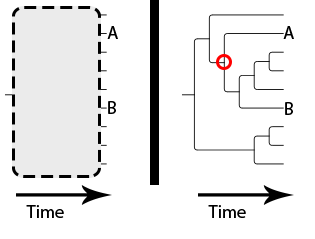
\includegraphics[scale=0.75]{phylogeny03}
\centering
\caption[Unknown phylogeny]{An illustration of unknown phylogeny. Since the phylogenetic information under the shaded box is typically not known, the point of divergence (red circle) can't be determined.}
\label{fig:phylogeny03}
\end{figure}
In this example, two related organisms A and B are compared with an attempt to determine when and how a specific trait was gained or lost by one of the organisms. This may be useful, for example, when attempting to estimate the relative importance (due to conservation over many generations) of some trait. Without the phylogenetic information (under the shaded box) it may not be possible to identify the point in their evolutionary history at which the two organisms diverged, making time estimates difficult or impossible.

Another major downside to in vivo evolutionary experiments is that they are slow. For example, the well-known E. coli Long-Term Evolution Experiment (LTEE) by Profesor Lenski at Michigan State University has been ongoing since February of 1988 and only passed generation 50,000 in 2010, 22 years later\footnote{\url{http://myxo.css.msu.edu/ecoli/celebrate50K.html}}. As an alternative to in vivo experiments, in silico evolutionary experiments are well-suited to the task of studying reductive evolution. Generations of organisms may be evolved within a very short time period, and a full "fossil record" of each lineage may be kept on disk for further analysis. 

The in silico tool Aevol has a realistic artificial chemistry model which was developed specifically to study genome structure. It contains tools to analyze the robustness, fitness, and evolvability of digital organisms over time.  In this thesis, Aevol is used to perform experiments in silico evolution in order to determine the effects of several different conditions on the genome of a simulated ``wild type'' bacteria. The changes to the size and structure of the genome will be carefully examined in the following pages. 

This chapter serves as the introduction to the thesis and the research problem being faced. In Chapter~\ref{ch:02background}, some necessary background information is provided on reductive evolution, in silico evolution in general, and Aevol in particular. Chapter~\ref{ch:03methods} describes the experimental setup. Chapter~\ref{ch:04results_discussion}
provides the results and analysis of the experiments of this thesis, and Chapter~\ref{ch:05conclusion} presents the conclusions drawn from this work. 



\chapter{Background}\label{ch:02background}

In this chapter, some of the theoretical background information required for this thesis is examined. An overview of experimental evolution is given before moving on to a discussion of Aevol, the specific tool that was used in this thesis. The chapter closes examining how Aevol can be used to study reductive evolution and by discussing the current state of the literature surrounding reductive evolution.  

\section{Properties of Genomes}
This section describes some general properties of evolutionary theory which will be required for this thesis. Some general properties about evolution were covered in Section~\ref{ch:01intro} and now some more specific properties of genomes will be examined, as these will play a large role in the coming experiments. 

\subsection{Evolvability}\label{subsec:evolvability}
Evolvability is usually defined as the ``prospective ability [of a population] to produce new mutations that can be used in adaptive evolution in the medium to long term'' \cite{brookfield2009evolution}. In other words, a system has evolvability if ``mutations in it can produce heritable phenotypic variation''\cite{doi:10.1098/rspb.2007.1137} and, critically, that this is not simply having a large amount of genetic diversity but rather \textit{adaptive} diversity which provides some benefit. 

There is, then, a link between evolvability and selection, since it is of course in an organism's best interest to be able to adapt to new environments or situations. Evolvability should, therefore, be selected for, though it may not be obvious how, say, a random mutation which confers no immediate benefit (but which increases evolvability) may be selected for. One possibility might be the idea of ``genetic hitchhiking'', in which an allele changes its frequency not because it is itself under selection but because it is near another gene which \textit{is} under selection. Intuitively, if an ``evolvability trait'' arises which provides no immediate fitness benefit but which confers some benefit to offspring, eventually this trait will also increase in frequency as the fitness advantage conferred on the offspring causes them to be selected. The idea is discussed at greater length by Arenas et al.~\cite{selectionEvolvability}. 

In real-world scenarios, it can be difficult to calculate evolvability for two reasons. First, evolvability can usually only be measured over evolutionary timescales. It isn't usually possible to look at a genome and determine its evolvability, since this involves looking at its offspring and examining their fitness (or some other phenotype) in some environment. Second, the stochastic nature of mutations makes it very difficult in real-world scenarios to compare two populations, since one has to separate the noise of random mutations from the signal of evolvability~\cite{selectionEvolvability}. 

\subsection{Robustness and Antirobustness}\label{subsec:robustness_antirobustness}
Robustness is broadly defined as the ability of an organism to withstand disruptions or perturbations without affecting its phenotype. There are differing kinds of robustness, as well: one may describe robustness in terms of mutational robustness\textendash which describes the extent to which an organism's phenotype is not affected by stochastic mutational events\textendash or one may speak of environmental robustness, which describes the ability of an organism to maintain its phenotype in diverse environments with little or no loss in fitness. 

Also important is the idea of antirobustness, wherein an organism may actually \textit{thrive} on such perturbations. This has been suggested as a possible method of minimizing the effects of \textit{Muller's ratchet}, wherein deleterious mutations accumulate in a population as a result of genetic drift\cite{Gordo2137}. A large number of initially-deleterious mutations may provide fodder for selection to fix more beneficial mutations in the population\cite{doi:10.1186/s12862-019-1507-z}.

There is, then, a seeming trade-off between robustness and evolvability. The more robust a system is, the less phenotypic variation is generated by random mutation events, and thus less evolvability. However, a key factor is to distinguish between genomic and phenotypic robustness; a strong phenotypic robustness promotes structural evolvability, as the likelihood that a mutation is deleterious is smaller in populations with more robust phenotypes. For a fuller discussion, see Wagner et al.~\cite{doi:10.1098/rspb.2007.1137}.

\subsection{Fitness}\label{background:fitness}
In population genetics, ``fitness'' can relate to either the genotype or the phenotype and denotes the contribution of an individual to the gene pool of the next generation; it is usually discussed in terms of \textit{absolute fitness} and \textit{relative fitness}~\cite{cutter2019primer}. The absolute fitness $W$ of a genotype is the level of proportional change in the abundance of that genotype from one generation to the next. So if, for example, a genotype in generation $t$ exists with abundance $n(t)$, then $n(t+1) = W*n(t)$. 

Relative fitness, on the other hand, describes the change in genotype \textit{frequency}, i.e. the fraction of all chromosomes in the population that carry a particular allele. For a population of size $N$, if a genotype's frequency at time $t$ is given by $p(t) = n(t)/N(t)$, then $p(t+1) = \frac{w}{\bar{w}}*p(t)$, where $\bar{w}$ is the mean relative fitness in the population. This implies that $\frac{w}{\bar{w}}$ is proportional to $\frac{W}{\bar{W}}$. 

\section{Reductive Evolution}\label{reductive_evolution}
Reductive evolution is the process by which organisms evolve to have a smaller average genome size than their ancestors via a pattern of gene loss~\cite{wilcox2003consequences}. This has been observed both in free-living bacteria such as \textit{Prochlorococcus} as well as endosymbiotic bacteria living inside host cells (e.g. \textit{Buchnera aphidicola} in aphids). Patterns consistent across most cases of reductive evolution are: a reduced GC content (impacting protein stability), gene loss, low non-coding to coding DNA ratios, and rapid sequence evolution~\cite{Batut.2014}. Some of the hypothesized mechanisms behind reductive evolution include: limits imposed by the effective population size (i.e. ``Muller's ratchet'', described below), the ``Black Queen Hypothesis'', and environmental adaptation. 

In Muller's ratchet, organisms with smaller effective population sizes, such as \textit{Buchnera aphidicola}, may lose genes because deleterious mutations accumulate in a population due to the smaller population size not allowing for enough variability. In the absence of recombination, these deleterious mutations become fixed in a population. The idea was originally put forth by H.J. Muller~\cite{MullersRatchet}.

The Black Queen Hypothesis suggests that genes may be lost when some subset of the bacteria in a community is able to provide the same function as the lost genes for the benefit of the rest of the community, allowing some bacteria to lose those genes and receive the benefit from others~\cite{morris2012black}. 

Lastly, one other proposed hypothesis among many has been environmental adaptation. For example, many reduced strains of the marine cyanobacteria \textit{Prochlorococcus} live in nutritionally-poor surface waters. It has been suggested that perhaps genome reduction is an adaptation which allows reduced strains to conserve precious nutrients~\cite{rocap2003genome, dufresne2005accelerated}. 

\section{Experimental Evolution}
As discussed in Chapter~\ref{ch:01intro}, in vivo experiments, although sometimes more realistic, have their own set of difficulties. Some examples of these difficulties include recreating challenging environmental conditions (e.g. simulating the open ocean in a laboratory) and identifying and/or simulating the multiple selection pressures acting on genomes in the real world~\cite{Batut.2013}. These challenges add enormous difficulty and complexity to conducting proper experiments and isolating the specific factors which lead to particular outcomes. 

In silico evolution simulates the evolution of organisms in software, thus allowing for far greater control and analysis of the environment and other experimental conditions. In contrast to in vivo experiments, a greater amount of control is also available with regard to the way organisms may interact, reproduce, and evolve. For example, a genome may be created completely from scratch or an existing genome may be fed into the simulation. Reproduction rates can depend on overall fitness, on relative fitness, or some other criterion. 

Factors such as the mutation rates or selection pressure are then parameters for the model and may be kept constant or allowed to vary over time. Given that these are parameters of the system, they may be tightly controlled, leading to a clearer picture of the factors influencing different outcomes. An underlying deterministic model can also allow for a reconstruction of the system from any given point, allowing one to easily create a record of events, including phylogenetic trees. 

Although there are certainly limitations to using in silico evolution (see Section~\ref{limitations}), overall in silico experimental evolution is a valuable tool for studying the underlying mechanisms of evolution when real-world experiments would be prohibitively time-consuming or expensive.

Many silico evolution tools have been used to test various aspects of evolution, and several formalisms exist to represent the process. In a ``sequence-of-nucleotides'' model, genomes are represented by a string of characters representing base pairs. Other formalisms include the ``gene network model'' in which genes are nodes in a connected graph, as well as the ``digital organisms'' model, in which software programs representing organisms fight for CPU time. Examples of the latter type include Tierra~\cite{Tierra-Ray} and Avida~\cite{Avida-Ofria}, which were some of the first in silico evolution tools. DOSE, an ecology-conscious method of checking for heterozygosity (variation within a population)~\cite{Castillo-DOSE} is a more recent example of in silico experimental evolution. For a more comprehensive review, see~\cite{Mozhayskiy-In-Silico-Review}. 
 
\section{Aevol}
Aevol follows a ``sequence-of-nucleotides'' model~\cite{Batut.2013} in which organisms are simulated with a binary genome which can either be generated at random or input as a previously-generated sequence. Aevol essentially consists of a repeated iteration of three main steps: 1) decoding the genome of these organisms to produce artificial proteins, 2) selecting the most fit individuals and 3) reproduction of these fittest individuals with possible variations (mutations, rearrangements, etc.). The sections below examine each of these steps in greater detail.

\subsection{Why use Aevol}

The in silico tool Aevol was developed to ``study the evolution of the size and organization of bacterial genomes in various scenarios''\cite{Batut.2013}. The program has also been expanded upon and tested in a variety of scenarios over the years (e.g. \cite{parsons2011selection}, \cite{misevic2012effects}, \cite{Miramontes.2016}). Some examples of experiments in which Aevol was the primary mechanism of in silico experimental evolution include: testing the predictability of evolution with high mutation rates as in viruses~\cite{beslon:hal-01577115}, determining whether selection is able to overcome evolution's drive towards more complex organisms~\cite{Liard.2018}, examining the role of mutators in reorganizing the genome in order to overcome mutational load~\cite{doi:10.1186/s12862-019-1507-z}, examining the effects of population shape on levels of cooperation~\cite{Miramontes.2016}, modeling regulatory networks~\cite{sanchezdehesa:hal-01502737} and more. 

As an in silico experimental evolution tool, Aevol embodies several of the advantages of in silico evolution in general. There is a ``fossil record'' of each generation, experimental conditions are tightly controlled, and experiments are easily repeatable. The encoding/decoding strategy of Aevol follows a biologically realistic model, in the sense that there are many degrees of freedom between an organism's genome and its proteome. Many genes may encode for very simple proteins (e.g. if the genes contain the same or similar sequences), and by contrast, overlapping genes may code for complex proteomes.

In the following sections, the in silico experimental evolution tool Aevol will be examined in greater detail. 

\subsection{Aevol's Architecture}
Aevol's three main steps\textemdash decoding the genome, selection, and reproduction\textemdash are illustrated in Figure~\ref{fig:aevol_overview01} and are discussed in greater detail in the following sections. 

\begin{figure}[H]
	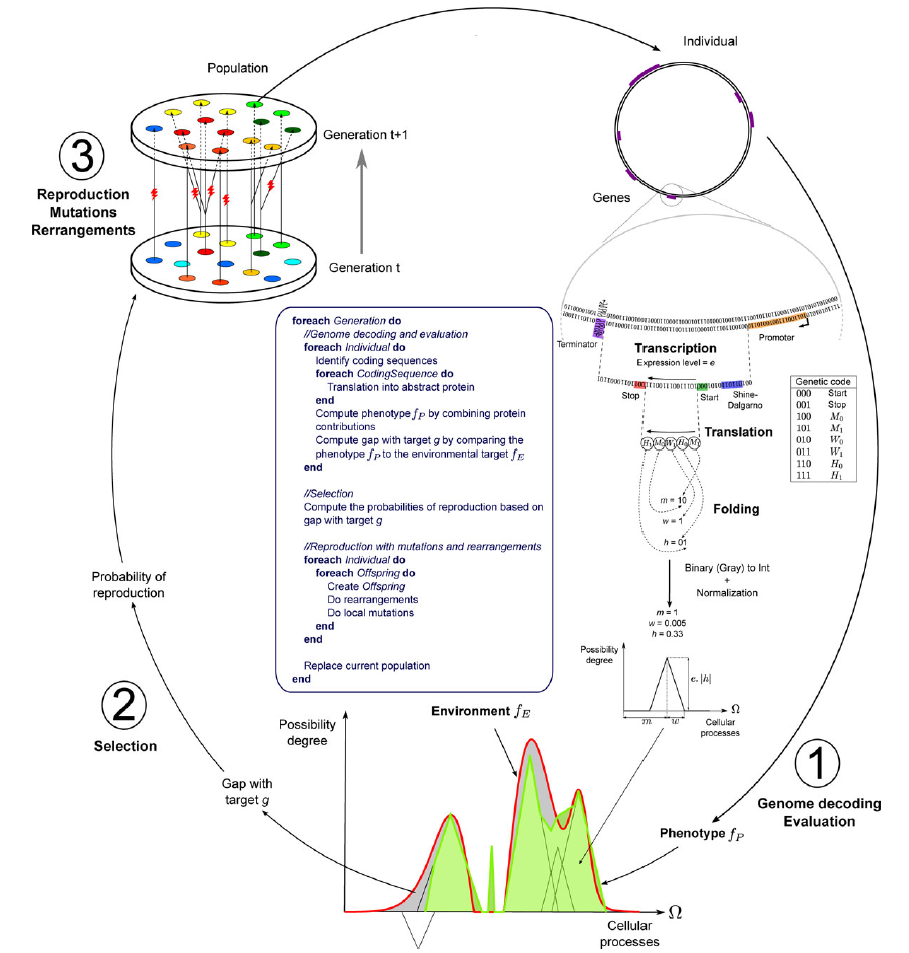
\includegraphics[width=\textwidth,height=\textheight,keepaspectratio]{aevol_overview01}
	\centering
	\caption[Overview of Aevol's architecture.]{Overview of Aevol's architecture, from~\cite{Batut.2013}. In step 1, the binary genome of the organisms is decoded and the resulting phenotype (bottom, in green) is matched up against an environmental target function (red line). In step 2, the probability of reproduction is calculated for each organism, based on its fitness (gap between the environment $f_E$ and its phenotype). In step 3, the next generation is created based on the probabilities from step 2, along with random mutations, rearrangements, etc.}
	\label{fig:aevol_overview01}
\end{figure}
\subsubsection{Decoding the Genome}\label{subsec:aevol_decoding}
In Aevol, a genome consists of a string of binary characters where 0 is complementary to 1. Each organism in the population has a double-stranded circular genome which is either generated randomly or which was provided as input. To decode the genome and produce the phenotype, the sequence is searched for transcribed regions. Transcribed regions are denoted by promoter and terminator sequences. The promoter sequence is a sequence whose Hamming distance $d$ is within $d_{max} = 4$ mismatches of the predefined consensus sequence $0101011001110010010110$. Terminators are sequences which can form a stem-loop structure with a stem size of 4 bases and a loop length of 3 bases (i.e. $abcd$***$\overline{dcba}$ where a is complementary to $\overline{a}$, b is complementary to $\overline{b}$, etc.). Lastly, the initiation and termination signals are sought, which are simply Shine-Dalgarno-like signals (i.e. $011011****000$ to start and $011011****001$ to stop). Lastly, an expression level $e$ is assigned to each coding region, following the formula $e = 1 - \frac{d}{d_{max} + 1}$ where $d$ is again the Hamming distance between the coding region and the consensus sequence given above and $d_{max}$ is the maximum allowable distance (i.e. 4). 

Once an initiation sequence is found, the following bases are read three at a time (codon by codon) until a stop codon (by default $001$) is found. If a stop codon is not found, then no protein is produced. Since a transcribed region may have multiple initiation signals, operons are therefore allowed. The codons following an initiation signal encode for three parameters according to the genetic code given in Figure~\ref{fig:aevol_overview01}: $m$ (mean), $w$ (half-width), and $h$ (height), which together define a triangle representing a ``cellular process''.

A cellular process is simply an abstract representation of some phenotypic function and is represented by the ordered set $\Omega = \left[ a,b \right] \subset \mathbb{R}$. Together, these cellular processes make up the organism's proteome. To keep things simple, $\Omega$ is a one-dimensional space in the interval $\left[0,1\right]$, i.e. a ``cellular process'' is simply a real number, and the genomic encoding of each cellular process determines the function $f(x) : \Omega \rightarrow \left[0,1\right]$. The mean $m$ gives us the specific cellular process in the range $\left[0,1\right]$. The width $w$ describes the ``scope'' of the process, i.e. the \textit{pleiotropy} of the process, meaning the subset of the protein that is in the interval $ \left(m - w, m + w\right) \subset \Omega$ . The height determines the degree of possibility of the process, i.e. its relative strength.

The codons are read one after the other and their Gray codes\footnote{A binary encoding such that two successive values (e.g. 2, 3) only differ by at most one bit (e.g. 0011, 0010). See \cite{doran2007gray} for an overview.} are used to compute the real numbers $m$, $w$, and $h$ as follows. Each parameter ($m$, $w$, $h$) is assigned two codons in the genetic code (see Figure \ref{fig:aevol_overview01}), for example $w_0 = 010$ and $w_1 = 011$. Any $w_0$ codons become a $0$ in the Gray code, and vice versa with $1$s. So if, for example, when reading the coding sequence, the codons $w_1$, $w_0$, $w_1$, $w_0$ are read, the Gray code becomes $1010$, which is 12 in decimal. This is done for $m$, $w$, and $h$, and the resulting values are then normalized to be in the proper range. $w$'s range is specified in the parameter file (as \texttt{MAX\_TRIANGLE\_WIDTH}), $h$ must be in the range $\left[-1,+1\right]$ (indicating that both activating and inhibiting processes are allowed) and $m$ must be in the range $\left[0,1\right]$ (the range of $\Omega$). 

Given the fact that there are likely multiple coding sequences in a genome, several triangles (cellular processes) are translated from the genome, each parameterized by its own $m$, $w$, and $h$. These triangles form the phenotypic function $f_P$. \textit{Fuzzy logic} is used to find the overall contribution of each cellular process, using the Lukasiewicz fuzzy operators\footnote{See \url{https://en.wikipedia.org/wiki/Lukasiewicz\_logic} for an introduction.}. Roughly speaking, the activating proteins are added up, as are the inhibiting proteins, and the difference between these two totals represents the final function $f_P$. More formally, if $f_i$ is the possibility distribution of the $i$-th activator protein and $f_j$ is the possibility distribution of the $j$-th inhibitor protein, then the phenotype of the individual is defined as:
\begin{equation*}
f_P = max\left(min\left(\sum_{i}^{}f_i(x),1 \right) - min\left(\sum_{j}^{}f_j(x),1 \right) ,0\right)
\end{equation*}

\subsubsection{Selection}\label{subsec:aevol_selection}
After the genome is decoded, the organisms are tested for their fitness. Fitness in Aevol is related to the gap between the phenotype of a sequence $f_P$ and the environmental  target function $f_E$, as illustrated in Figure \ref{fig:aevol_overview01}. This environmental target function $f_E$ is a user-defined set of Gaussians which are specified in a parameter file, with each Gaussian being identified by three parameters: its height, its location along the axis, and its width. The difference between the phenotype (as calculated above) and the environmental function is the ``metabolic error'', labeled $g$ in the figure and is more formally defined as:  $g = \int_{a}^{b} f_E(x) - f_P(x) dx$. The idea is illustrated in Figure~\ref{fig:aevol_fitness01}

\begin{figure}[H]
	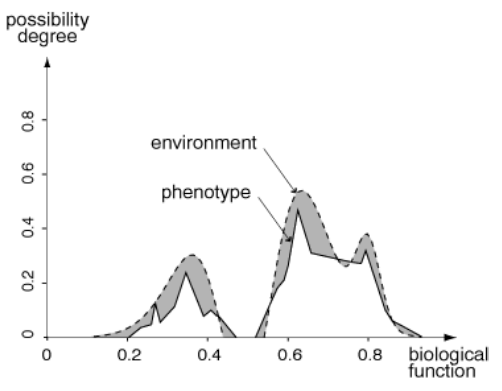
\includegraphics[scale=0.5]{aevol_fitness_description01}
	\centering
	\caption[Overview of Aevol's concept of fitness.]{Overview of Aevol's conception of fitness, from \cite{knibbe:tel-00482375}}
	\label{fig:aevol_fitness01}
\end{figure}

Aevol contains several selection schemes, but here only the \texttt{fitness\_proportionate} scheme will be considered, since this was the only selection scheme employed in these experiments. In this scheme, the probability of reproduction for each organism $i$ is proportionate to its fitness, namely:
\begin{equation*}
P(\text{reproduction}) = \frac{e^{-k * g}}{\sum_{i=1}^{N} e^{-k * g_i}}
\end{equation*} 
where $k$ is a user-definable parameter which determines the selection intensity and $g$ is the metabolic error.
\subsubsection{Reproduction}\label{subsec:aevol_reproduction}
Once the fittest organisms in the population are found and their probabilities of reproducing are calculated as described in the previous Section, new organisms are produced. This is done for each potential parent organism by drawing from a multinomial distribution with the probability of reproduction given above. The population size $N$ is kept constant and a record of each generation is kept so that the phylogenetic lineages can be recreated. Since the population size is held constant, this implies that a single organism with a high probability of reproduction may produce multiple offspring and an organism with low probability of reproduction may produce none.

When new organisms are created and their genomes are copied from their parent organisms, it is at this stage that some of the driving forces in evolution occur, namely the possibility for variation through mutation, indels, and frameshifts. Offspring will receive their parents' genome but their genome may be subject to perturbations due to stochastic effects. Mutation rates are set in the parameter file and include point mutations, insertions and deletions (indels), and rearrangements (duplication, deletions, translocations, and inversions).

The mutation, indels, rearrangement, etc. events are carried out by first determining the number $\mu$ of such events which will occur, based on the mutation rate specified in the parameter file and drawing from a binomial distribution (e.g. $B(L, \mu_\text{point})$ for point mutations, $B(L, \mu_\text{large deletions})$ for large deletions, etc. where $L$ is the size of the genome). Then a random point (or points, in the case of e.g. rearrangement) is chosen and the event is carried out, with the order of these events shuffled randomly. 

\section{Analyzing with Aevol}\label{sec:aevol_analysis}

Once the experiments have completed, Aevol by default produces several statistics files which include information about genome size, the percentage of coding DNA, number of genes, average metabolic error, and many other statistics. It further includes a number of post-treatments that allow one to analyze specific individuals or the population at large, including tools for determining robustness, evolvability, coalescence, and the lineages. 

One of the key features of Aevol is the ability to look back in time at the ''archaeological record'' of previous organisms, which is stored on disk, in order to perform various analyses. This is primarily done with a myriad of post-treatments'', i.e. supplementary programs. These post-treatments generally require a \texttt{lineage} file, which is a file generated by Aevol that shows a record back in time of the line of descent for an individual. One may specify either the best-ranked individual (i.e. the fittest) or a specific individual by their unique identification number. The basic idea is illustrated below in Figure~\ref{fig:lineage01}. 

\begin{figure}[H]
	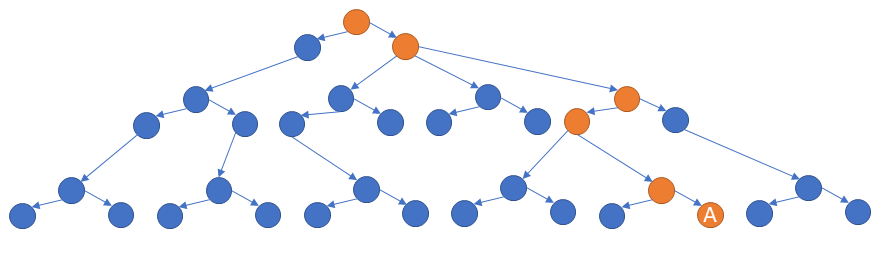
\includegraphics[width=\linewidth]{lineage01}
	\centering
	\caption[Lineage basic illustration.]{A basic illustration of a lineage. The ancestors of the individual (labeled `A') can be traced back through the previous generations for all of its ancestors (all in orange).}
	\label{fig:lineage01}
\end{figure}


\section{Related Work}\label{related_work}

%TODO Add population aspect of in silico experimental evolution - waiting on clarification from Berenice 5/20/2020 - Update 5/26/2020 never got a response. Turning it in as is. 

Much work has already been done in the field of reductive evolution and in silico experimentation, and this section will look at the current state of the literature. 

\subsection{Reductive Evolution}\label{related_work:reductive_evolution}
Regarding the influence of selection on reductive evolution, Liard et al. showed in~\cite{Liard.2018} that selection for fitness is not necessarily enough to overcome the tendency of organisms to become more and more complex. They describe the existence of a ``complexity ratchet,'' which characterizes this tendency of organisms to increase their complexity as being irreversible once the organisms have reached a certain complexity level. In their words:
\begin{quote}
	``Since gene deletion is obviously deleterious $\left[\text{in this scenario}\right]$, the only available evolutionary path for already complex organisms is a headlong rush toward increasing complexity by acquiring new genes. Hence the ratchet clicks, further widening the fitness valley that separates the current genome from a simple one, soon making it so wide it is very unlikely to be crossed."
\end{quote} 
Echoing the findings of Knibbe et al.~\cite{Knibbe2007} and performing in silico experiments with Aevol they found, however, that limiting \textit{robustness} can overcome the tendency of organisms to become more and more complex, because this places an upper bound on the amount of information that an organism can transmit in its genome. Limiting robustness by increasing the mutation rate forced gene elimination despite the fitness loss because it lowered the information content of the genome. A mutation rate of even $\mu = 10^{-4}$ resulted in nearly 40\% of their organisms developing a simpler genome.

Batut et al.~\cite{Batut.2014} investigated many of the different hypotheses which seek to explain the mechanisms behind reductive evolution (some of which were discussed in Section~\ref{reductive_evolution}), as evidenced in the marine cyanobacteria \textit{Prochlorococcus}. Among these explanations are: limits imposed by population size and ``Muller's ratchet,'' high mutation rates, the ``Black Queen Hypothesis'', and environmental adaptation. Batut et al. found that generally Muller's ratchet could explain the reduced genome size in endosymbiotic bacteria but that it was not enough to explain the reduction seen in \textit{Prochlorococcus} due to its large effective population size\textemdash some strains of \textit{Prochlorococcus} are estimated to have effective population sizes of up to $10^9$.  

Regarding the ``Black Queen Hypothesis,'' in which members of a (bacterial) community are able to reduce their genome size because other members of a community provide the lost functionality, Batut et al. found that this hypothesis was difficult to test for but suggest it may be a useful explanation for the evolution of endosymbiotic consortia.  

Given the previous discussion on high mutation rates and their impact on limiting robustness (and thus complexity), a discussion and focus on the last criterion of Batut et al., environmental adaptation, closes this section. Given the nutrient-poor environmental conditions in which \textit{Prochlorococcus} is often found, it has been suggested that perhaps the loss of genes is adaptive, since any superfluous genes (such as those required to ``respond to variation in nutrient concentrations'') inherently carry a fitness cost. However, several gene losses observed in \textit{Prochlorococcus} suggest that the reduction was not adaptive, however. For example, many DNA repair genes were lost, and the immediate fitness benefits of such a loss are not obvious. 

Regarding genome structure, in the same experiments mentioned above, Knibbe et al.\cite{Knibbe2007} also found, via in silico experimentation, that the accumulation of non-coding DNA strongly depends on the mutation rate. This in turn affects the selection trade-off between reliably passing on the existing genome and having the mutational variability to adapt to new challenges.  Under higher mutation rates, their organisms closely resembled viral genomes in that they had almost no non-coding sequences. When the selection strength was larger, genomes were larger.  Another aspect of genome structure, namely gene density, was examined by Kuo et al. \cite{kuo2009consequences}, who examined the role of genetic drift on gene density (i.e. the ratio of the number of genes per number of base pairs) and found that, as the ratio of non-synonymous to synonymous substitutions increased, gene density varied much more greatly.
\subsection{Investigations in Experimental Evolution}

Koskiniemi et al.~\cite{koskiniemi2012} performed in vivo experiments on the bacterium \textit{Salmonella enterica} in which the effects on fitness of random deletions was measured. Some 25\% of the deletions actually caused an increase in fitness under some conditions, suggesting that there is a certain cost associated with having superfluous genes and thus gene loss may be selected for under certain conditions. In the usual race between the gene-preserving force of selection and the natural tendency of bacterial genomes towards deletion and streamlining, Koskiniemi suggests that perhaps it is sometimes a team effort. 

Liard et al. showed in their experiments with Aevol that complexity can arise in organisms in even the most simple of environments (a single triangular target function) and with the most basic beginnings (a single gene and protein)~\cite{Liard.2018}. They found that the complexity continues to increase, even when the resulting organisms are much less fit than the simpler ones, and that this complexity even overcomes selection. They also found that whether an organism would develop into a simple or complex organism was usually determined quite early in its evolution, around generation 10,000. Reasoning that genome compactness is a direct driver of mutational robustness, as Knibbe et al.~\cite{Knibbe2007} showed, and that more robust organisms can be selected over fitter organisms under heavy mutational stress as shown by Wilke et al.~\cite{wilke2001evolution}, they wondered if robustness could select for a more simplified genome. To test this, they changed the mutation rate to be exceptionally high (up to $\mu = 1e^{-4} *bp^{-1}*gen^{-1}$) and ran their simulations for another 100,000 generations, and the results confirmed their expectations: The higher the differential between the old and the new mutation rate, the larger percentage of organisms evolved a more reduced genome (up to 91\% in the case of a change from $\mu_\text{old}=1e^{-6}$ to $\mu_\text{new}=1e^{-3}$).

\section{Summary}
Connecting it all together, there is, then, a natural link between the amount of non-coding DNA, coding DNA, genome size, evolvability, robustness, and selection. As the amount of non-coding bases (and often therefore overall genome size) increases through natural mutational processes, these non-coding bases can nevertheless play a crucial role in increasing evolvability by being the fodder for new potentially beneficial mutations~\cite{Knibbe2007}. However, a trade-off exists because the increased \textit{mutational load} (i.e. the increasing cost of recurrent harmful mutations, as most mutations are) also carries a fitness cost. In a population whose effective population size is too small, these deleterious mutations accumulate, a phenomenon known as Muller's ratchet~\cite{MullersRatchet}.
\chapter{Methods}\label{ch:methods}
With an understanding of the basics behind us, in this chapter we provide an overview of our contributions and proposed solution.

\section{Contributions}

\section{Experimental Designs} \label{experimental_design}
To assist in determining which conditions might lead to reductive evolution, we need to isolate individual variables and change just one thing at a time in order to see what effect, if any, it has on the final genome. To that end, we designed and conducted a series of experiments in which a ``wild type'' genome was allowed to evolve in differing conditions for 500,000 generations before analyzing the results. To first create the wild type, a genome was generated randomly in Aevol which had at least one coding gene and which was allowed to evolve for 10 million generations in a non-varying environment. By the beginning of its use in our experiments, the wild type comprised 13,237 base pairs with 132 functional genes (i.e. genes which produce a gene product). We allowed the wild types to continue to evolve in the same environment in a total of 6 different conditions: with an increased/decreased selection strength, an increased/decreased mutation rate, and an increased/decreased population size. 

Additionally, a control condition was performed in which the wild type was simply allowed to continue to evolve for the 500,000 generations with no change in any of the above conditions. To minimize bias, for each condition we performed five runs each (i.e. 5 rounds of mutation up, 5 rounds of mutation down, etc.) each with a differing random seed to control for the deterministic effects of the pseudorandom nature of Aevol's stochastic processes. This lead to a total of 35 experiments, all of which were carried out on a cluster from bwCloud\footnote{\url{https://www.bw-cloud.org/}}. 

The resulting data was processed using a combination of Python\footnote{\url{https://www.python.org/}}, Pandas\footnote{\url{https://pandas.pydata.org/}}, and Jupyter Notebook\footnote{\url{https://jupyter.org/}}.  

\subsection{Inputs}
In Table \ref{table:parameters}, our parameter values for all input parameters may be found. Please note that for $\mu$, this represents the mutation rates for point mutations, small insertions, and small deletions. The rearrangement rates were not changed under any condition and were always $1e-6$ for duplications, deletions, translocations, and inversions. 

\begin{table}[h]
	\centering
	\begin{tabular}{|c||c|c|c|}
		\hline
		 & \multicolumn{3}{c|}{\textbf{Parameter}} \\
		\cline{2-4}
		\textbf{Condition} &$\mu$ & $k$ & $N$ \\
		\hline
		control & $1.00E{-7}$ & $1000$ & $1024$ \\
		\hline
		mutation up & $4.00E{-7}$ & $1000$ & $1024$ \\
		\hline
		mutation down & $2.50E{-8}$ & $1000$ & $1024$ \\
		\hline
		selection up & $1.00E{-7}$ & $4000$ & $1024$ \\
		\hline
		selection down & $1.00E{-7}$ & $250$ & $1024$ \\
		\hline
		population up & $1.00E{-7}$ & $1000$ & $4096$ \\
		\hline
		population down & $1.00E{-7}$ & $1000$ & $256$ \\		
		\hline
	\end{tabular}
	\caption[Table of parameters]{Table of input parameters. $\mu$ is the mutation rate, $k$ is the selection strength, and $N$ is the population size.}
	\label{table:parameters}
\end{table}
As can be seen in Table \ref{table:parameters}, only one parameter varied per condition in order to isolate potential influences. A multiplier of $4$ was chosen for the differing conditions relative to the control condition (e.g. $N_\text{population up} = 4096$ because $N_\text{control} = 1024$). In all conditions, the environment did not vary, and once the experiment was begun, the above parameters were held steady as well. 
\subsection{Evaluation Strategy}
In this section, we will examine what criteria we will be using to evaluate the results. The primary criteria will be examining the evolved genome's evolvability, robustness, and structure. 
\subsubsection{Robustness}
\subsubsection{Evolvability}
\subsubsection{Time to Coalescence}

\subsubsection{Statistical Significance of the Conditions}
Lastly, we need to determine whether the results of the condition (mutation up, selection down, etc.) were significantly different from the control condition, statistically speaking. To do this, we will evaluate the means of all seeds of the control condition for some test (e.g. robustness, evolvability, etc.) vs. the same for a different condition (e.g. mutation up) using the Wilcoxon signed-rank test. This is similar to a paired Student's t-test but is used when the distribution of the two samples cannot be assumed to be normally distributed. More precisely, we will use the Mann-Whitney U test, a nonparametric version of the Wilcoxon test which can be used when the sample sizes are different. The Mann-Whitney U test checks whether two independent samples were selected from populations having the same distribution. The test consists of the following steps:
\begin{enumerate}
	\item Assign numeric ranks to all observations
	\item Add up the ranks for the observations from the first sample
	\item The statistic $U_1$ for the first sample is given by:
	\begin{equation*}
	U_1 = R_1 - \frac{n_1*(n_1 + 1)}{2}
	\end{equation*}
	where $n_1$ is the sample size for the first sample and $R_1$ is the sum of the ranks from the first sample.
\end{enumerate}
The $U$ statistic for the second sample is computed analogously. We used the \texttt{Scipi.stats.mannwhitneyu} function to calculate this statistic as needed, which also calculated the p-value. 

\section{Expected Results}
%TODO Generate table of expected results similar to one in Berenice's thesis






\chapter{Results and Discussion}\label{ch:results_discussion}
This chapter presents the results of our experiments as performed according to the plan described in Chapter~\ref{ch:methods}. Section~\ref{results} provides the data and we then discuss these results in Section~\ref{discussion}. 

\section{Results}\label{results}
In this section we present the results of our experiments. We begin by presenting the results of our statistical analysis before moving on to show the results in various plots. It is of minor note that in many of the figures, a rolling window was used to smooth the values, resulting in many of the plots only showing data starting after a few thousand generations (often 10,000). It should be noted, however, that organisms were continuously evolved for 500,000 generations. 

\subsection{Genome Size}\label{sec:genome_size}
In this section we will examine the results of the different conditions, focusing on which, if any, lead to a reduced genome. Figure~\ref{fig:genome_size} presents the main findings regarding genome size. In the figure, the blue line shows the control condition and the other colors show the changed conditions: $\mu_+$/$\mu_-$ (mutation up/down), $k_+$/$k_-$ (selection up/down), and $N_+$/$N_-$ (population up/down). As can be seen from the figure, our expectations in Section~\ref{sec:expected_results} did not hold up, as all conditions actually \textit{increased} over their original size.
\begin{figure}[H]
	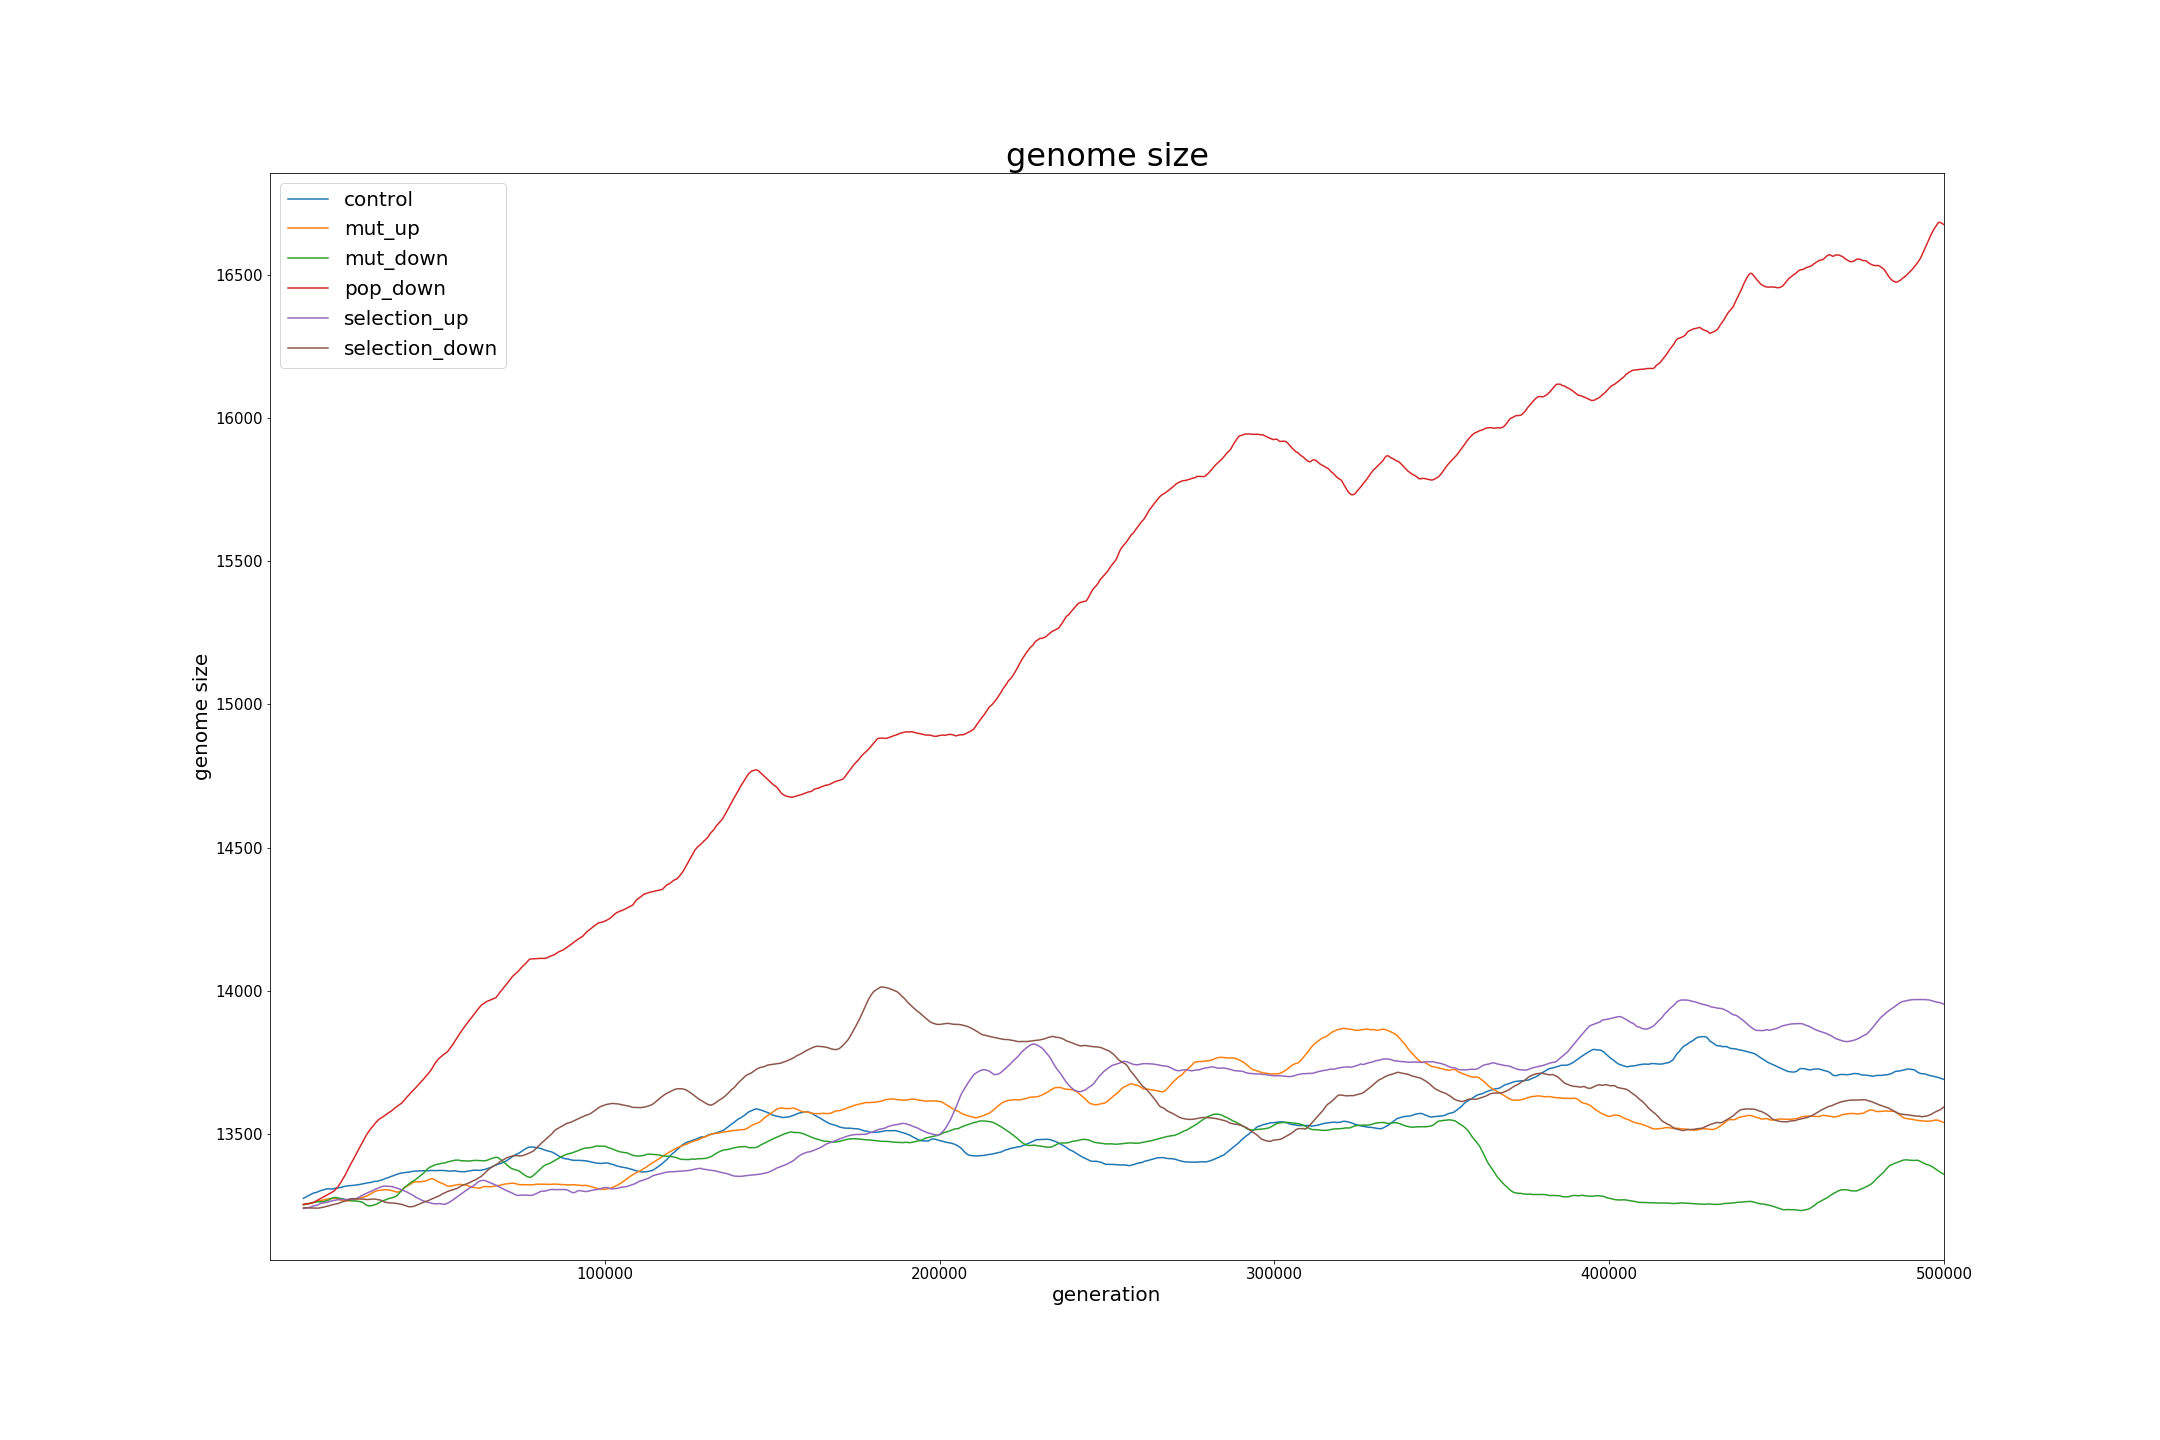
\includegraphics[width=\linewidth]{stat_fitness_global_mean_genome_size}
	\centering
	\caption[Genome size]{Genome size in number of bases of all conditions. Average taken across all five seeds for each condition.}
	\label{fig:genome_size}
\end{figure}
In fact the \textit{population down} condition had a runaway increase in the number of bases, reaching over 16,500 bases at one time, a 25\% increase over the original wild type's roughly 13,200 bp. Surprisingly, even after 500,000 generations it seems that the upper limit may still not have been reached. The statistical results are given below in Tables~\ref{table:genome_size_stats} and \ref{table:genome_size_mean_and_std_dev}, which show the mean and standard deviation among all five seeds.

\begin{table}[H]
	\begin{tabular}{|c|c|c|}
		\hline
		\multicolumn{3}{c}{\Large \textbf{Genome Size - Mean \& Std. Dev. (in bp)}} \\
		\hline
		 & \textbf{mean} & \textbf{standard deviation} \\
		 \hline
		 Control & 13537.031513461712 & 144.35113788568995 \\
		 \hline
		 $\mu_+$ & 13558.37415989583 & 155.0778470373894 \\
		 \hline
		 $\mu_-$ & 13410.74368980468 & 101.37610437279282 \\
		 \hline
		 $k_+$ & 13621.901103597776	& 229.63570760641895 \\
		 \hline
		 $k_-$ & 13614.663598682531 & 172.67504183409068 \\
		 \hline
		 $N_-$ & 15275.14939195188 & 950.2662434333312 \\
		 \hline
	\end{tabular}
	\caption[Genome size - mean and std. dev.]{Average genome size and standard deviation for all seeds and all conditions. }
	\label{table:genome_size_mean_and_std_dev}
\end{table}

\begin{table}[H]
	\centering
	\begin{tabular}{|c|c|c|}
		\hline
		\multicolumn{3}{c}{\Large Genome Size - Rank Sum \& P-Values} \\
		\hline
		& \textbf{rank sum U} & \textbf{p-value} \\
		\hline \hline
		$\mu_+$ & 110508011469.5 & 0.00000000000000 \\
		\hline
		$\mu_-$ & 71008638349.5 & 0.00000000000000 \\
		\hline
		$N_-$ & 16477791900.5 & 0.00000000000000 \\
		\hline
		$k_+$ & 100151680984.5 & 0.00000000000000 \\
		\hline
		$k_-$ & 88533681875.0 & 0.00000000000000 \\
		\hline
	\end{tabular}
	\caption[Genome size statistics]{Genome size statistics. Each condition is compared with the \textit{control} condition.}
	\label{table:genome_size_stats}
\end{table} 

The next most obvious observation is that of the remaining conditions, all but the \textit{selection up} condition (which had an an increase of 11\% over the control condition) ended up with fewer base pairs than the control condition, though all increased slightly over their starting point. Also noteworthy is that the mutation down condition appears to have had a steady increase in the number of base pairs until a maximum of just over 14,000 around generation 350,000 before having a fairly sharp decline back to nearly the original size. 

Examining the percent changed from the \textit{control} condition shown in Figure~\ref{fig:genome_size_percent_change} we see that at points, the \textit{mutation down} condition was nearly 5\% smaller than the \textit{control} condition. 

\begin{figure}[H]
	\centering
	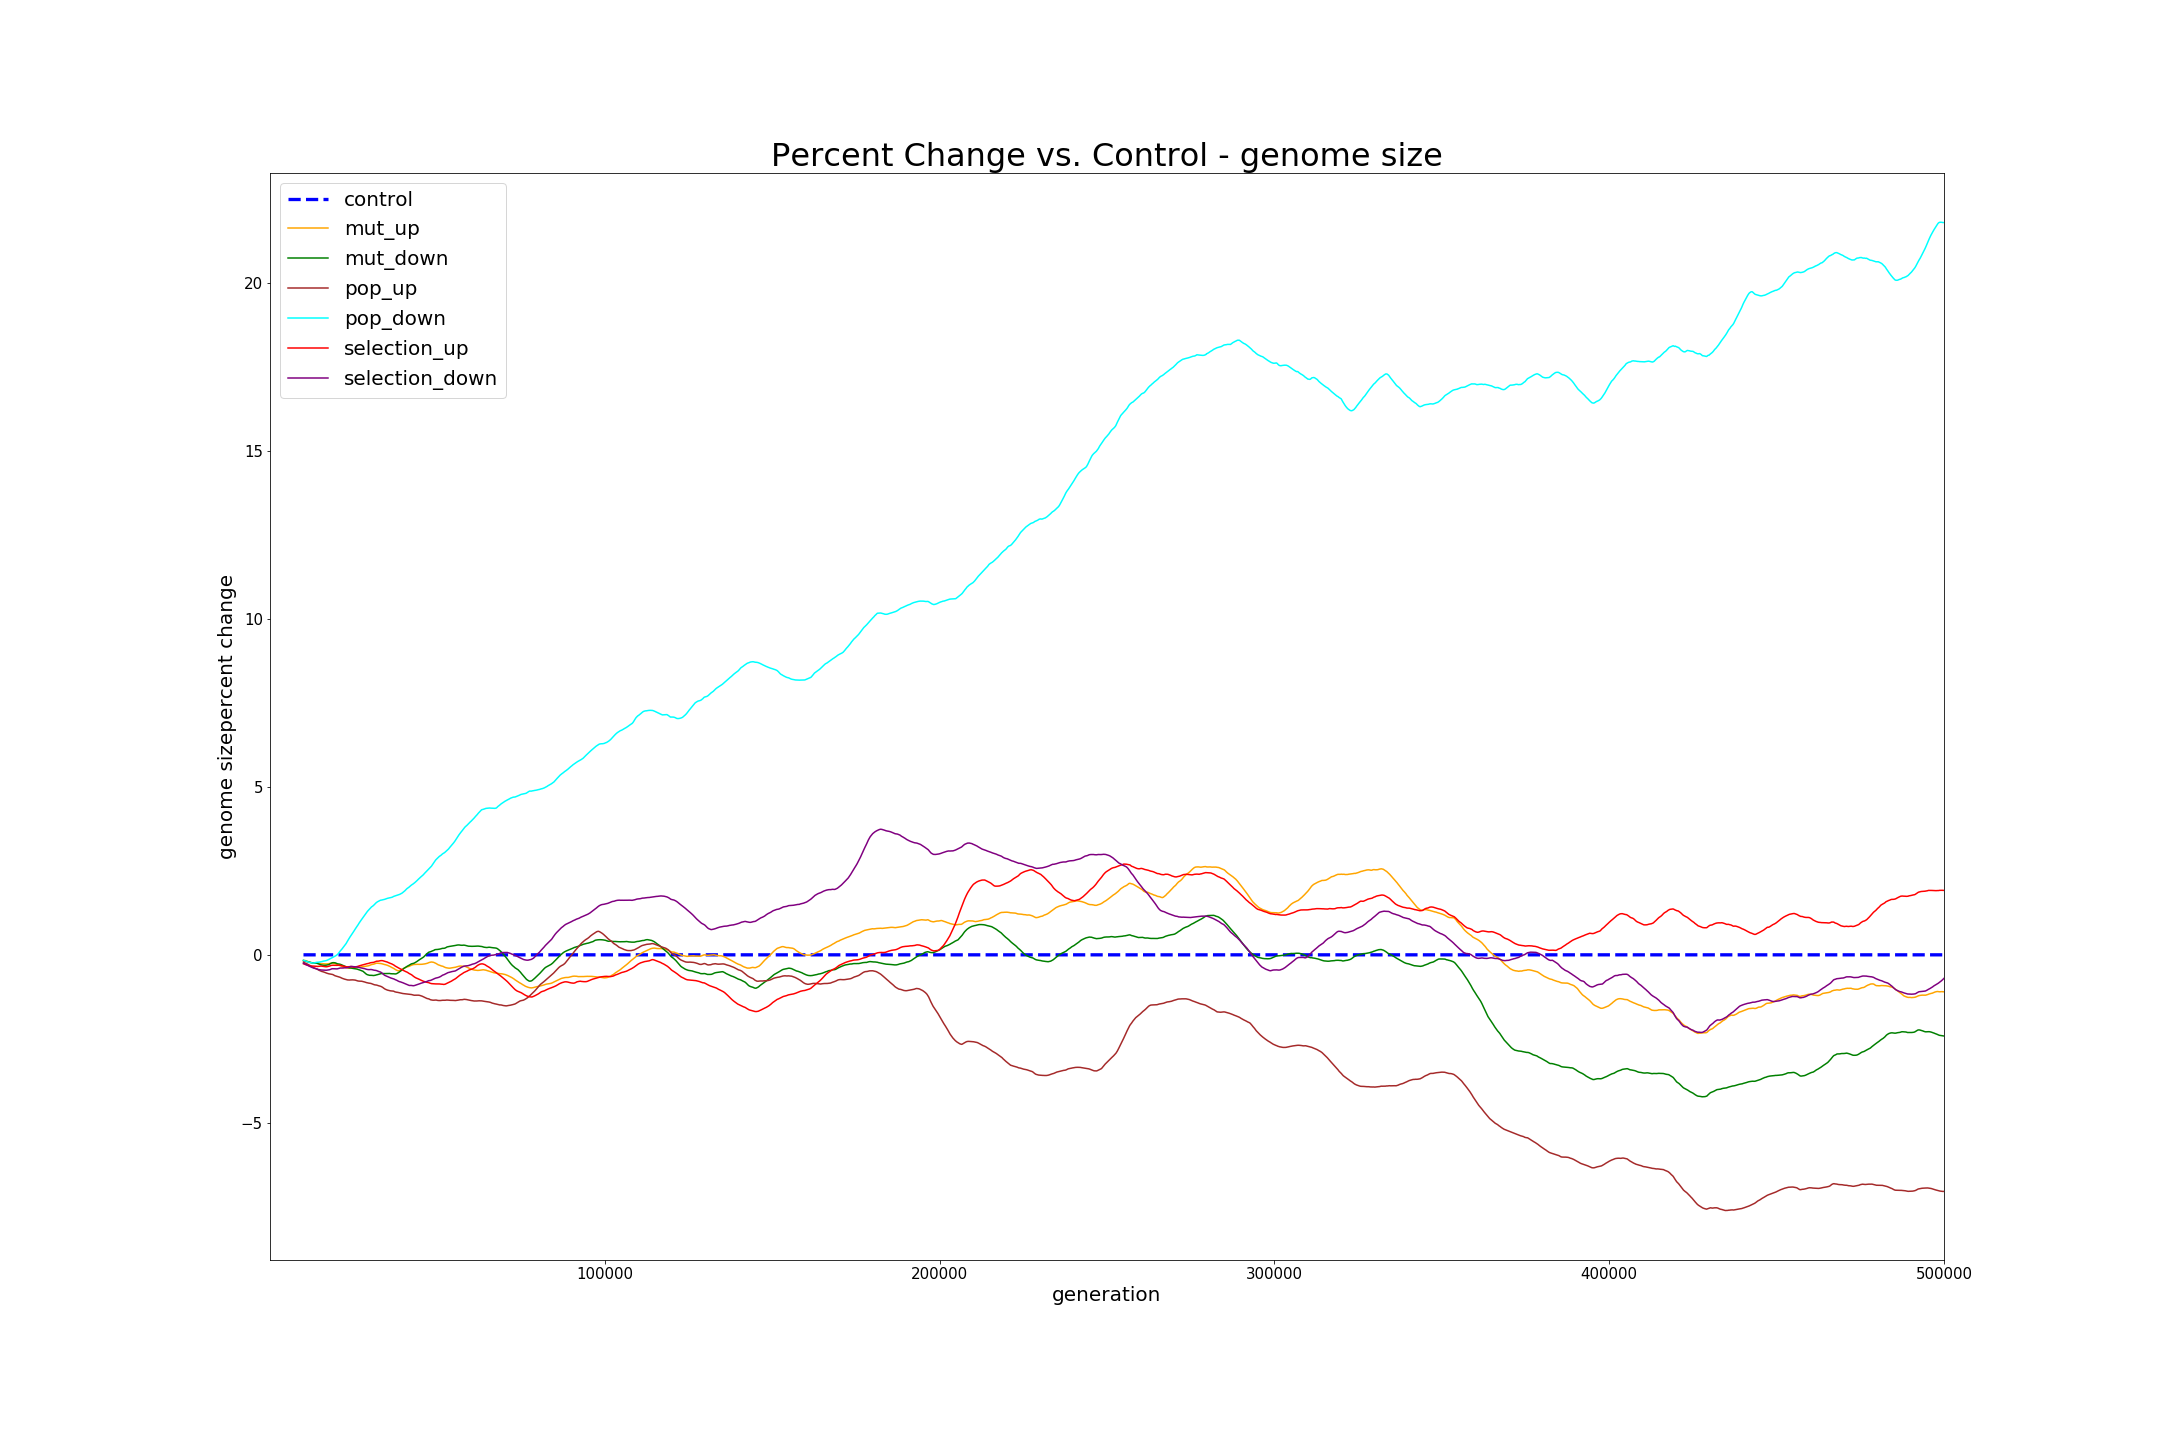
\includegraphics[width=\linewidth]{stat_fitness_perc_change_genome_size}
	\caption[Genome size - percent change]{Genome size's percent change from the \textit{control} condition.}
	\label{fig:genome_size_percent_change}
\end{figure}


\subsection{Metabolic Error and Fitness}
Figure~\ref{fig:mean_fitness_plot} shows the mean fitness of the population for the control, mutation up/down, and population down conditions. Selection up/down were excluded from this graph because they were significantly outside of the range of the other conditions and made the results impossible to graph, but they are included in Figure~\ref{fig:global_fitness_histogram}, a histogram of the results.

\begin{figure}[H]
	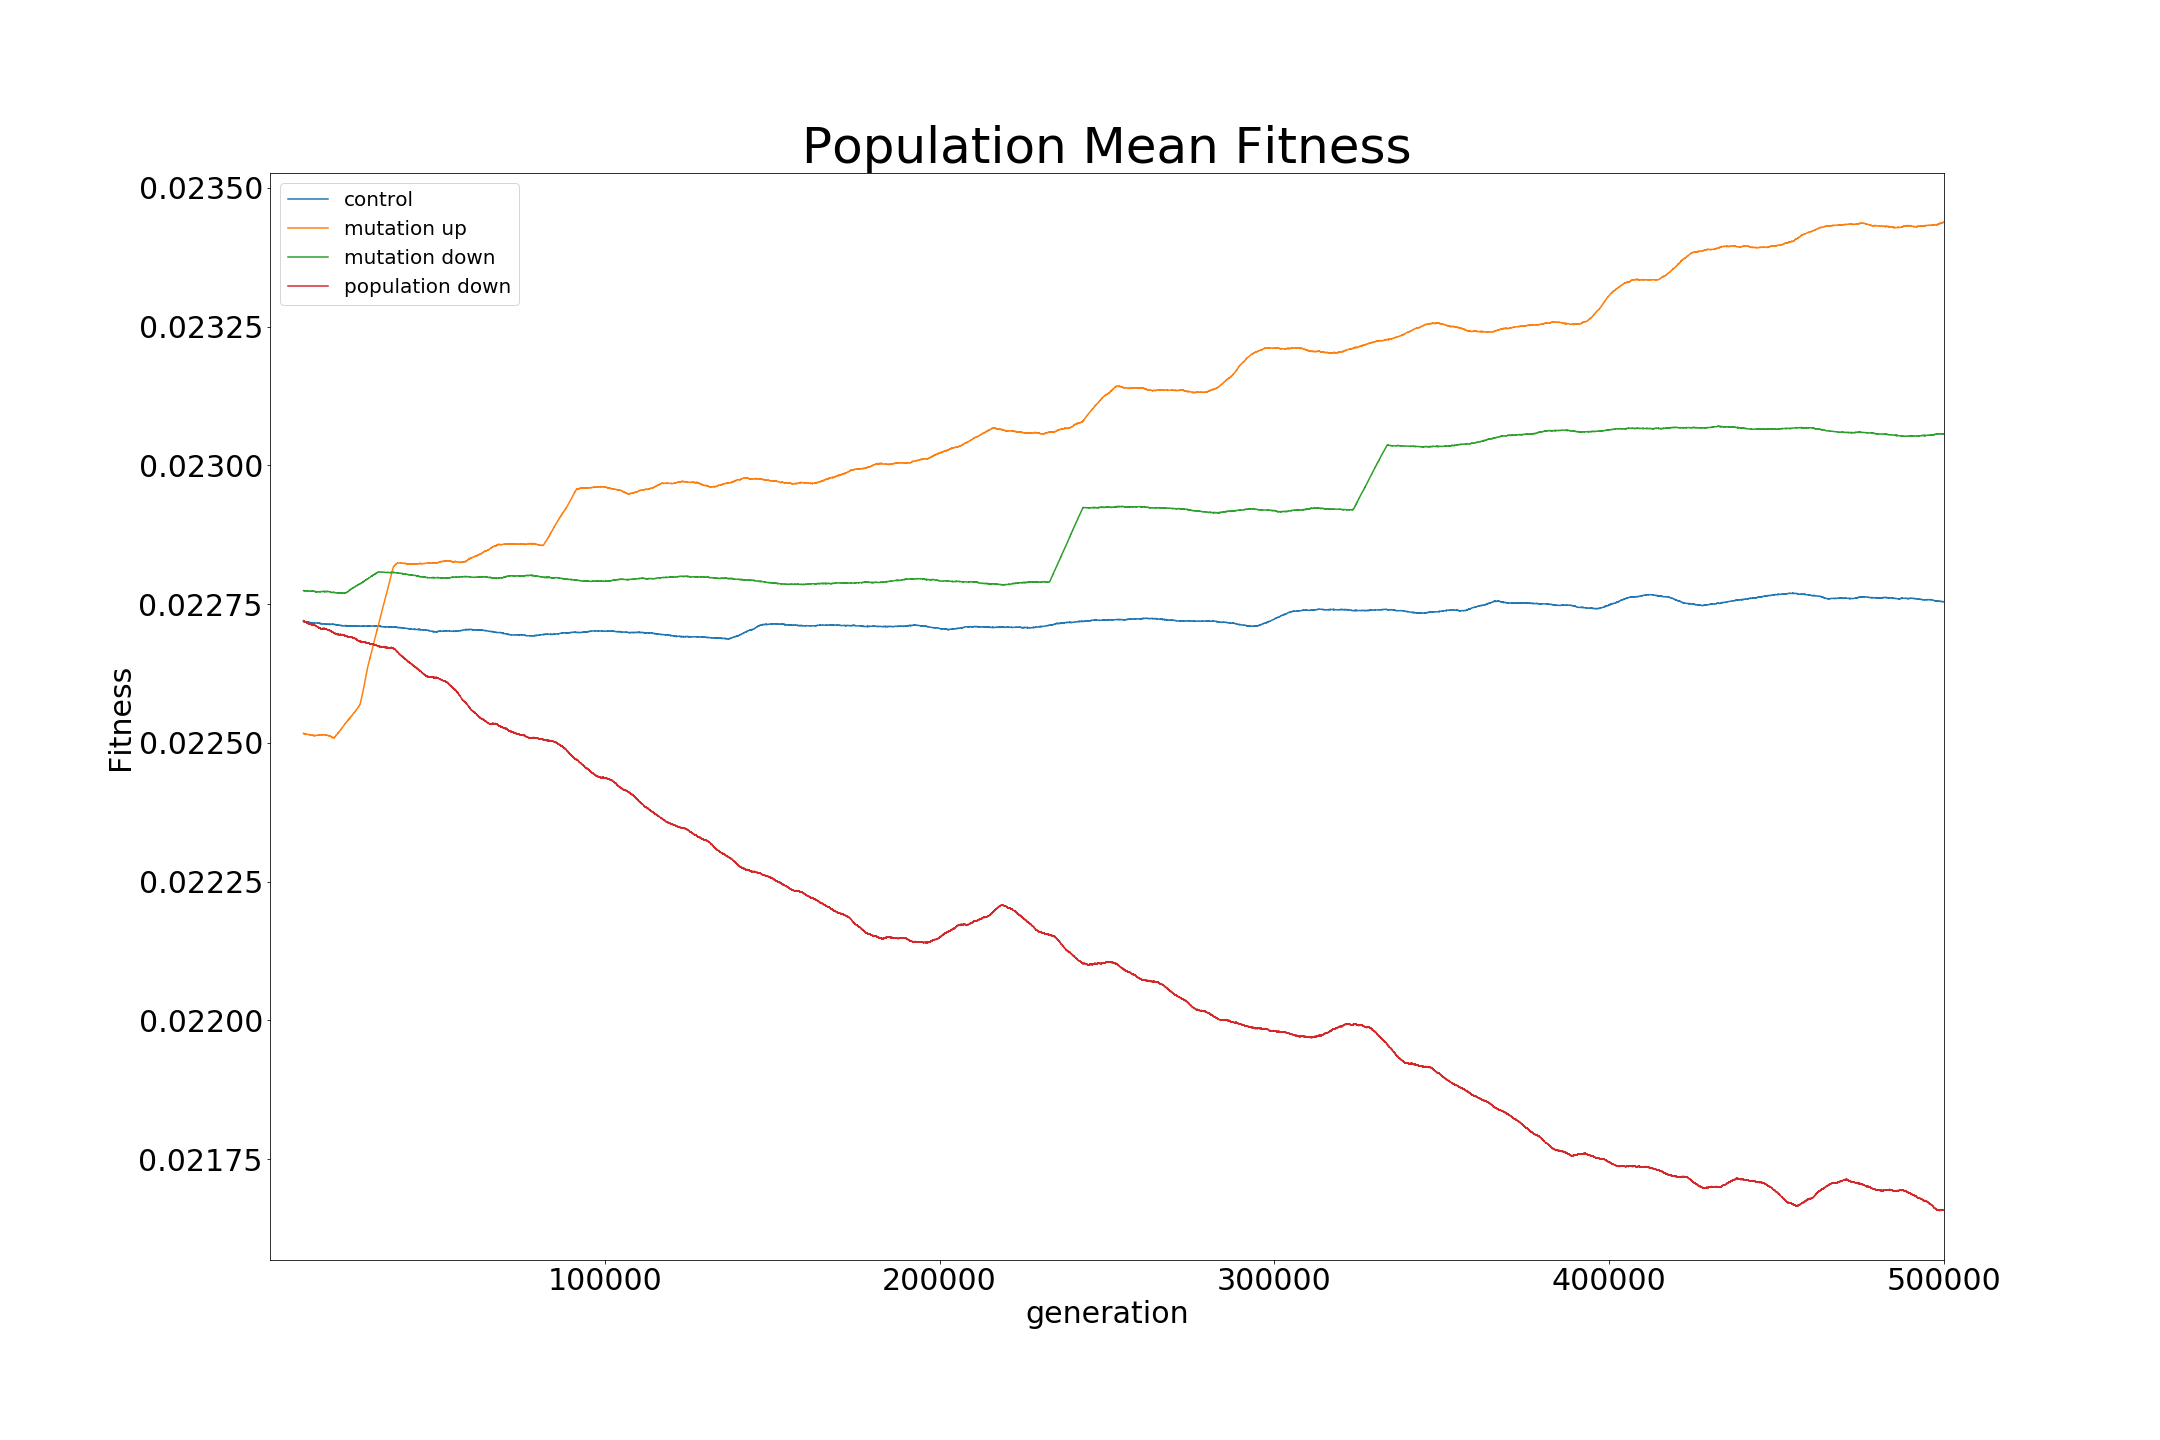
\includegraphics[width=\linewidth]{population_mean_fitness_chart}
	\caption[Mean fitness]{Plot of the mean fitness over time for the control, mutation up/down, and population down conditions.}
	\label{fig:mean_fitness_plot}
\end{figure}

We can see in the figure that the fitness of the control condition (in blue) consistently stayed at the same level, likely owing to the fact that the wild genotype had already been allowed to evolve for 10 million generations in this environment, so the phenotype closely lines up with the target before the simulations even began. Small fluctuations occurred due to mutations, insertions, etc. but since we were beginning with a clonal population of the best organism after 10 million generations in this environment, the average fitness remained steady. 

More interesting is the population down condition, where the average fitness in the whole population sharply declined, sinking to 4.5\% below the control condition at generation 500,000. It seems that with the smaller population size, genetic drift may be more strongly at work in continually increasing the gap between the phenotype and environmental function, as the lack of variety inherent in a smaller population causes a cascade of increasingly deleterious consequences. 

\begin{figure}[H]
	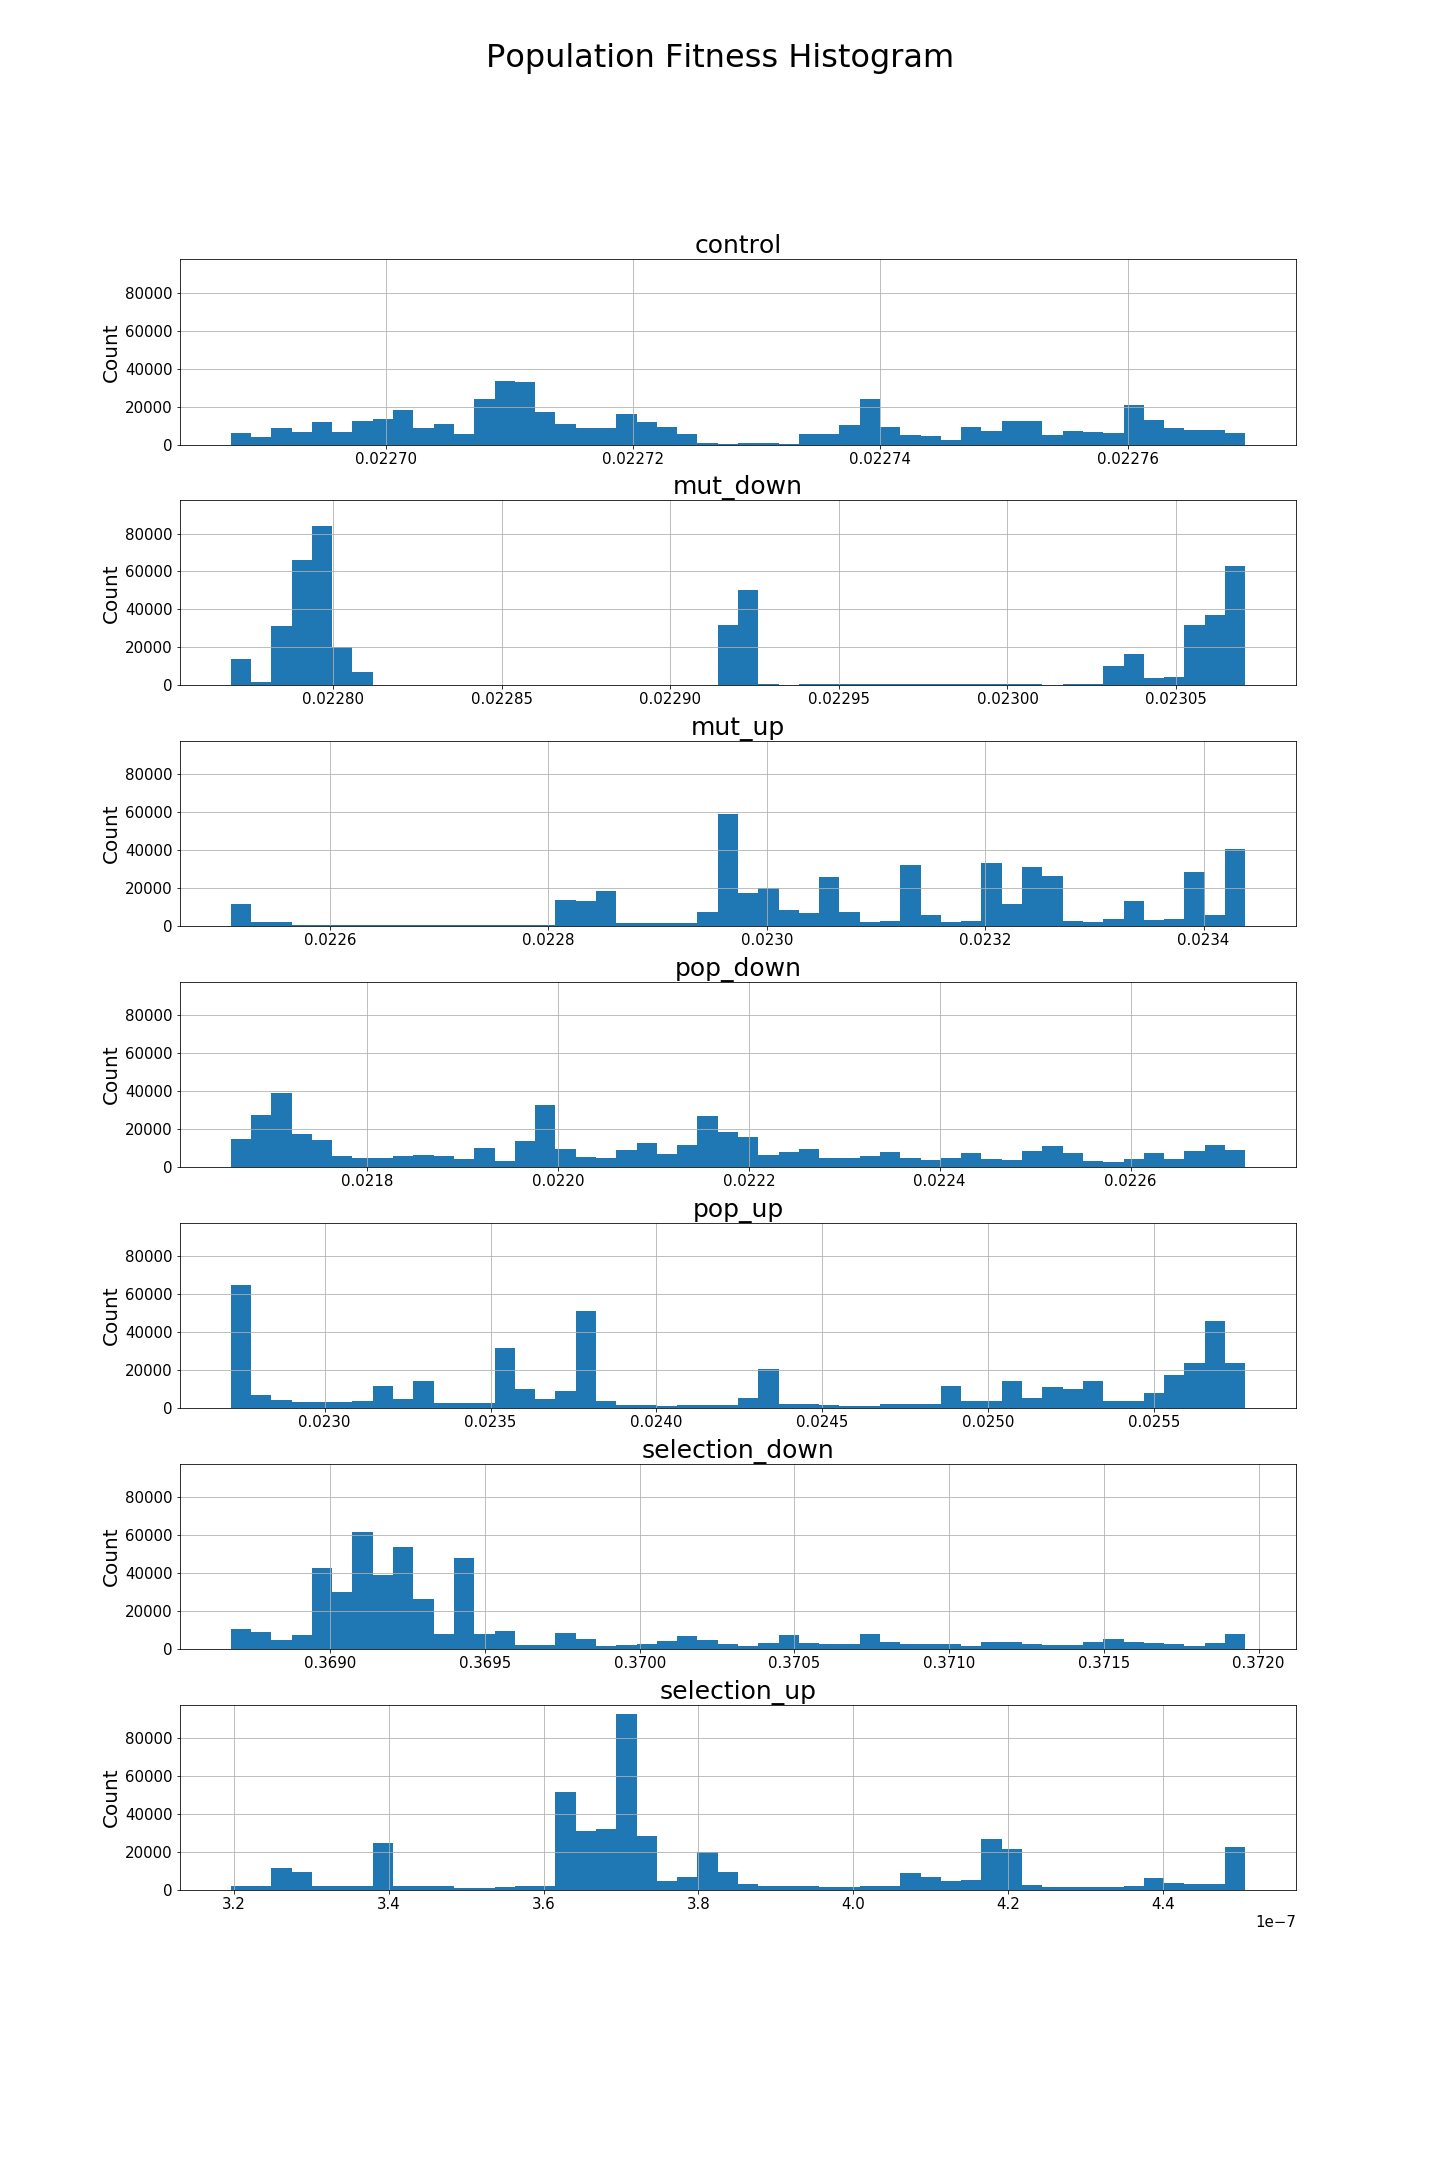
\includegraphics[width=\linewidth]{global_fitness_histogram}
	\caption[Mean fitness histogram]{Histogram of all conditions' fitness. Note that for the selection up condition, the scale is 1e-7. }
	\label{fig:global_fitness_histogram}
\end{figure}
Figure~\ref{fig:global_fitness_histogram} shows a histogram of all fitness values for all conditions. Although the \textit{mutation down} condition ended the simulations in the most similar position to the \textit{control} condition, Figure~\ref{fig:global_fitness_histogram} makes it clear that the \textit{control} condition remained much steadier throughout the simulation, regularly jumping from value to value, whereas the \textit{mutation down} condition, as expected, tended to hover at certain locations in between rarer mutation events. 

Figure~\ref{fig:mean_metabolic_error} shows the mean metabolic error across all seeds for the whole population over time with respect to each condition. 
\begin{figure}[H]
	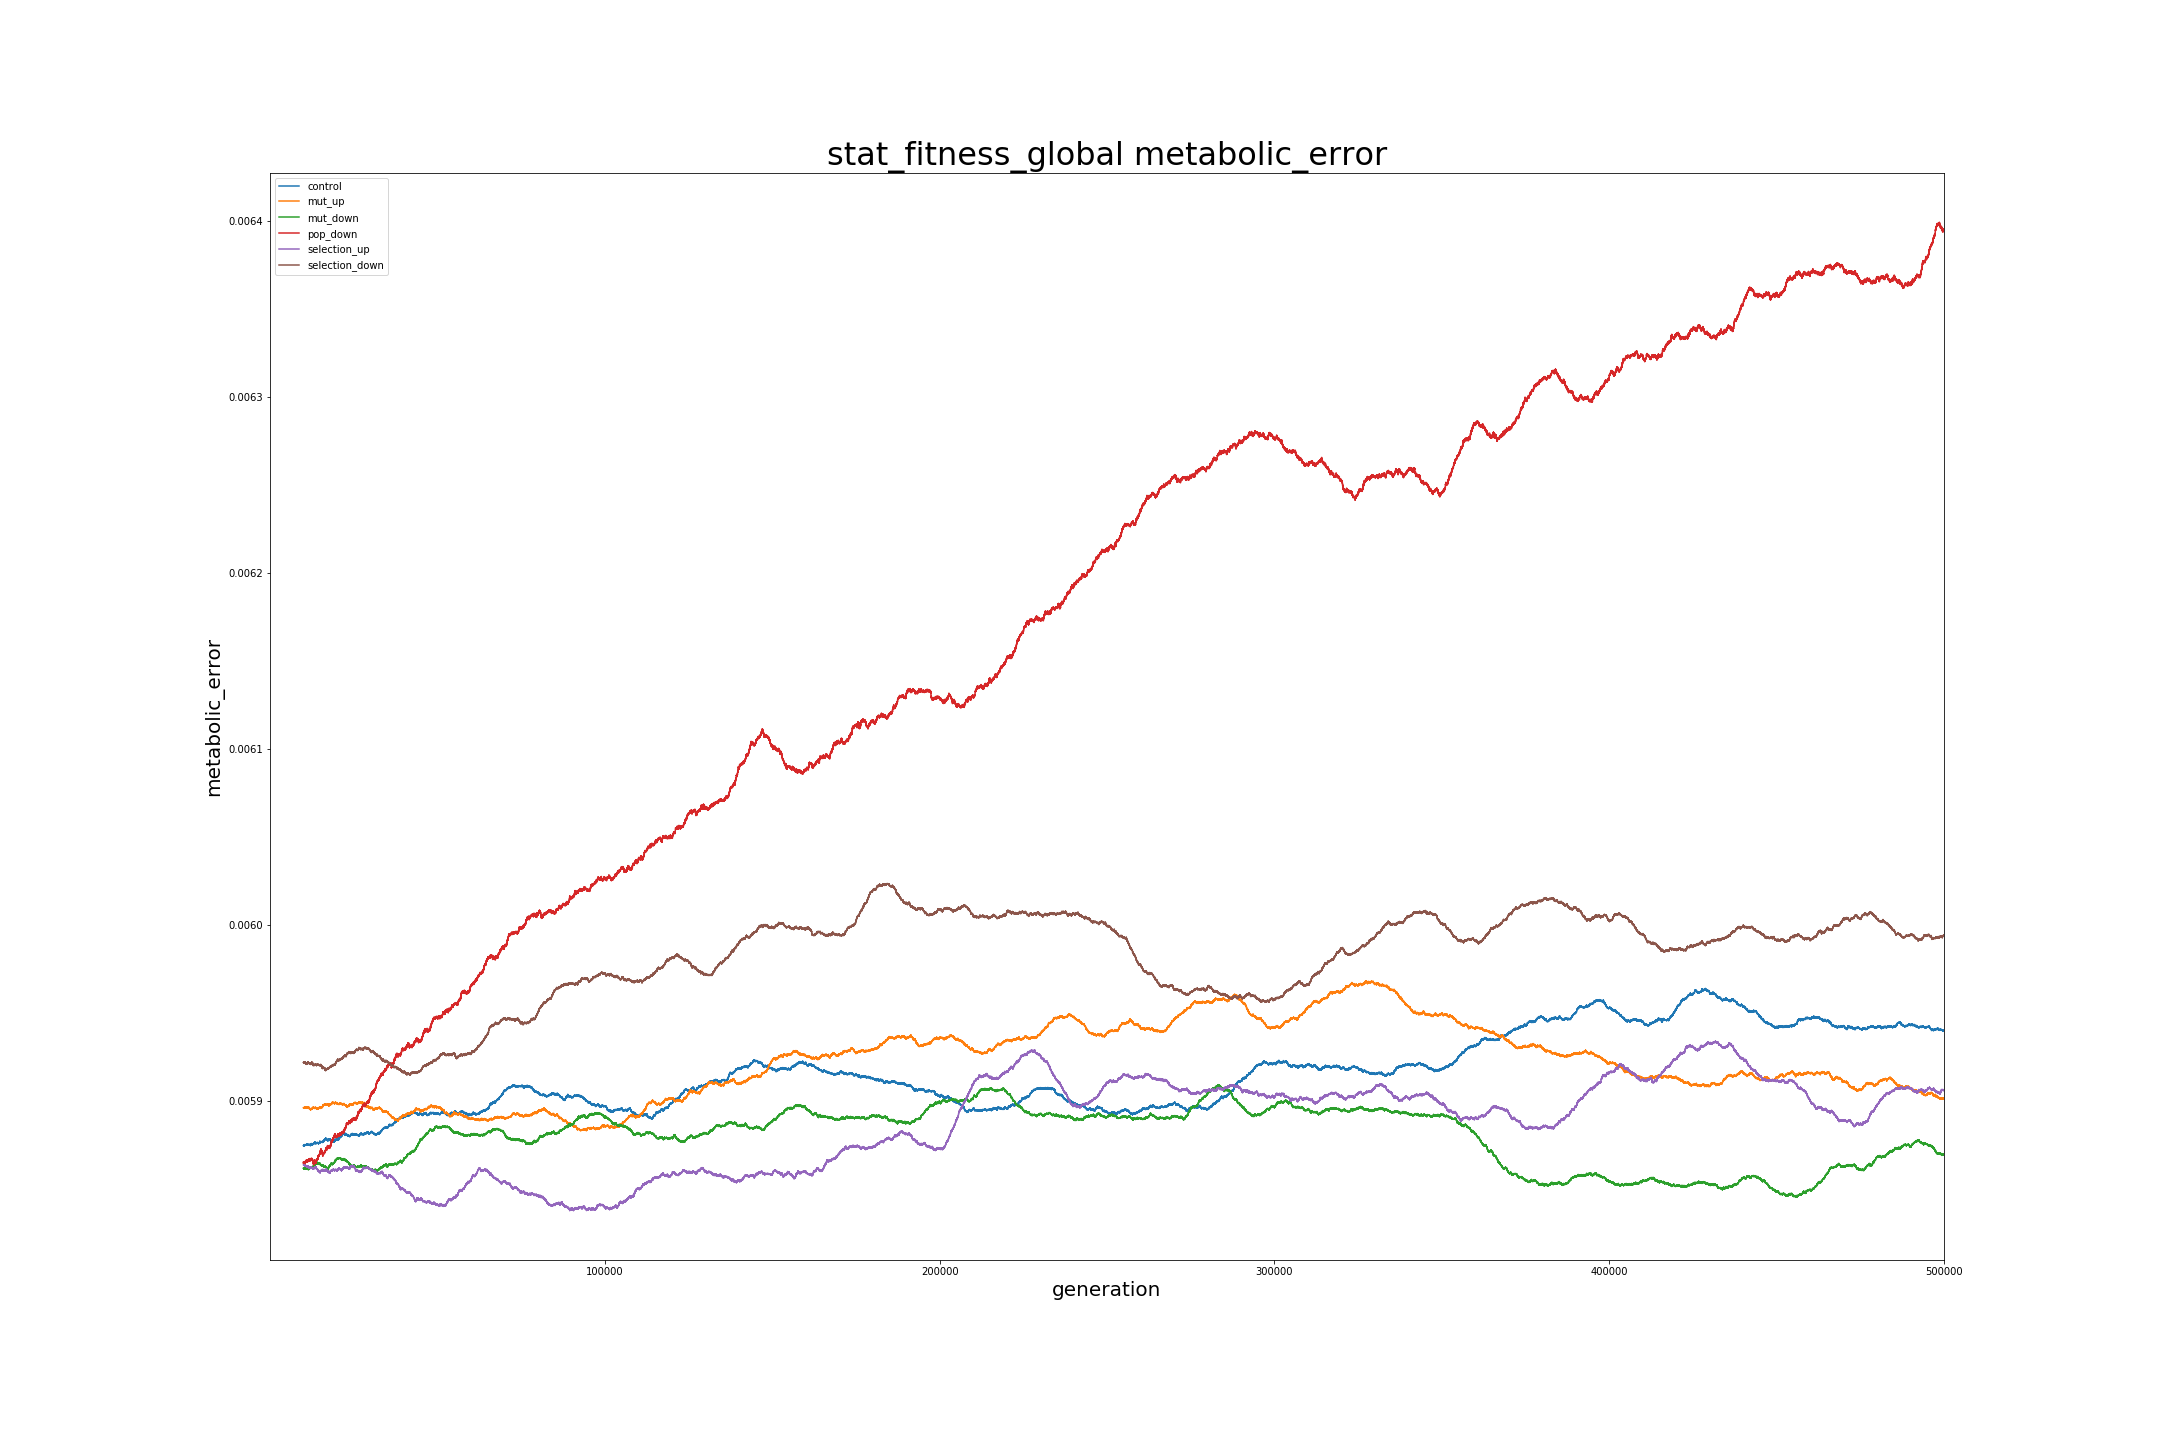
\includegraphics[width=\linewidth]{stat_fitness_global_mean_metabolic_error}
	\caption[Metabolic error]{Plot of the metabolic error over time for all conditions, average of all seeds}
	\label{fig:mean_metabolic_error}
\end{figure}

Table~\ref{table:fitness_means_std_dev} below gives the mean fitness scores for differing conditions. The selection up/down conditions seem to be somewhat anomalous.
\begin{table}[H]
	\centering
	\begin{tabular}{|c||c|c|}
		\hline
		\multicolumn{3}{c}{\Large \textbf{Fitness}} \\
		\hline
		& \textbf{mean} & \textbf{standard deviation} \\
		\hline \hline
		control & 0.022725416617759595 & 2.3443283583311204e-05 \\
		\hline
		$\mu_+$ & 0.02310700617283088 & 0.00021918255246890017 \\
		\hline
		$\mu_-$ & 0.022908786914463554 & 0.0001180940074554785 \\
		\hline
		$k_+$ & 3.803823317637301e-07 & 3.130503751740127e-08 \\
		\hline
		$k_-$ & 0.3695935240107418	& 0.0008101731945386823 \\
		\hline
		$N_-$ & 0.02209722426327717 & 0.00031042637566743275 \\
		\hline
	\end{tabular}
	\caption[Fitness means and standard deviations.]{Fitness means and standard deviations across all seeds. }
	\label{table:fitness_means_std_dev}
\end{table}

\subsection{Genome Structure}
In this section we examine the effects of the differing conditions on the structure of the genome as measured by the criteria in Tables~\ref{table:aevol_stats_genes_and_bp} and~\ref{table:aevol_stats_fitness_and_mutation}. 

\subsubsection{Non-coding DNA}
One important factor in genome structure is the amount of non-coding DNA, i.e. the number of bases which are part of a genome but which do not encode protein sequences. Aevol gives the number of bases which are not in any coding sequence, as well as the total genome size, so one may easily calculate this percentage. The results from our experiments are shown in Figure~\ref{fig:mean_non-coding_DNA}. Recalling genome size in Figure~\ref{fig:genome_size}, it seems that as the genome size of the population down condition rapidly expanded, most of those expansions were non-coding.
\begin{figure}[H]
	\centering
	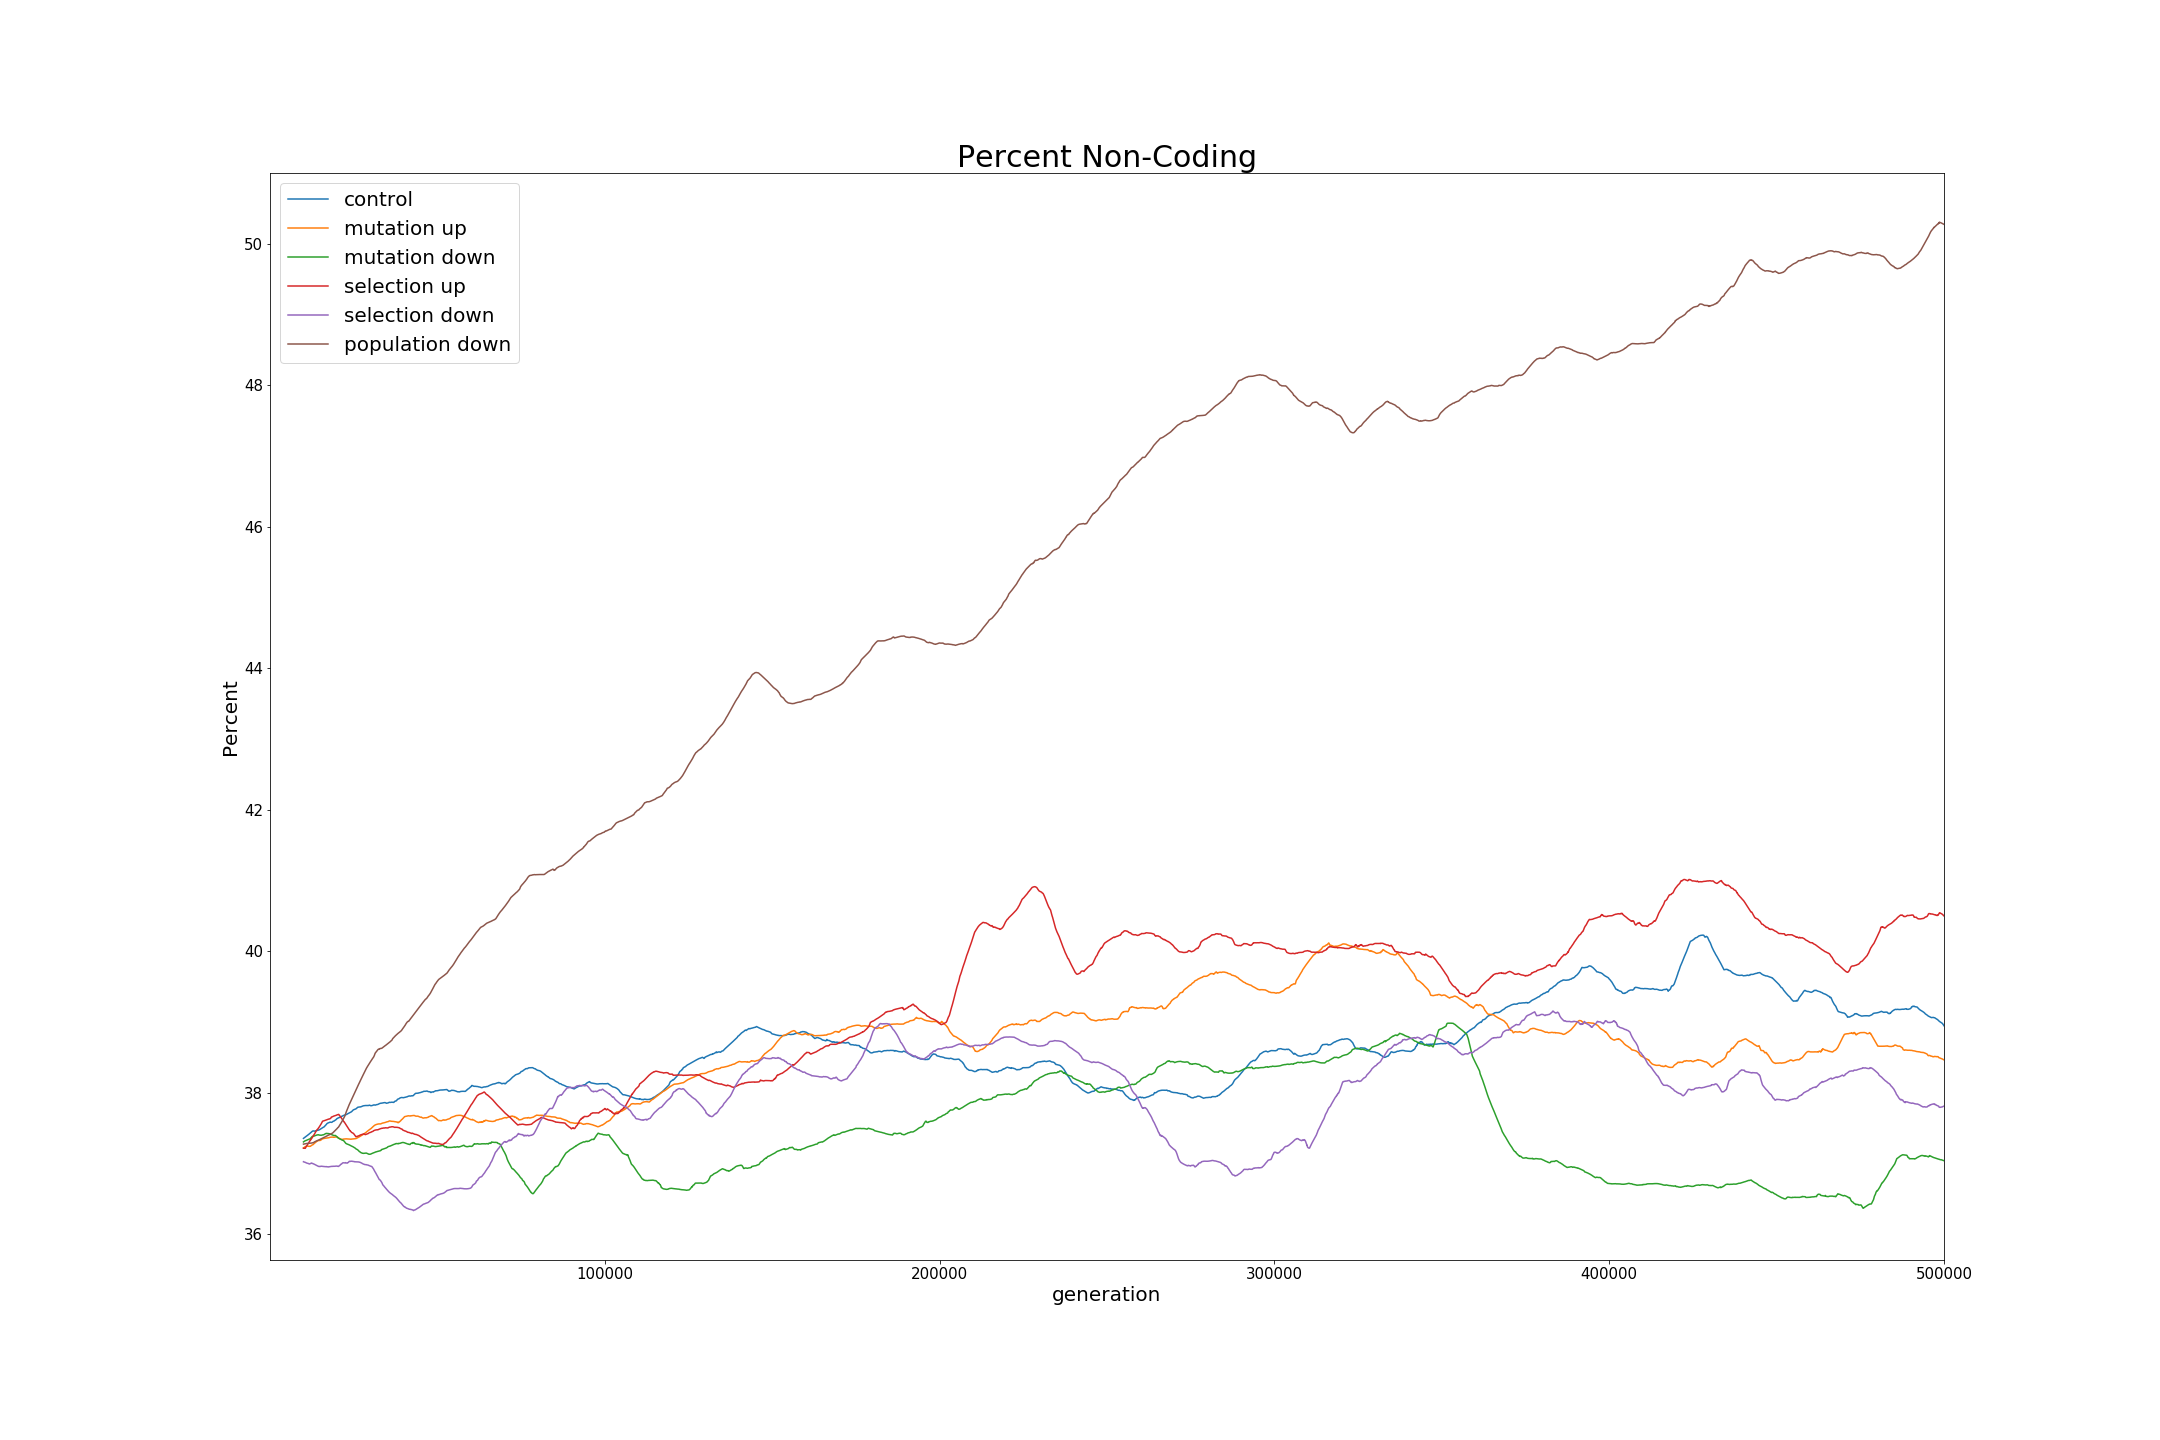
\includegraphics[width=\linewidth]{percent_noncoding}
	\caption[Non-coding DNA]{Plot of non-coding DNA over time for all conditions, average of all seeds.}
	\label{fig:mean_non-coding_DNA}
\end{figure}
By comparison, despite the \textit{selection up} condition's rapid decline in fitness, it did not acquire more than 1\% non-coding DNA. 

The average percentages of non-coding DNA are given in Table~\ref{table:non-coding_DNA_mean_and_standard_deviation} below. 
\begin{table}[H]
	\begin{tabular}{|c|c|c|}
		\hline
		\multicolumn{3}{c}{\Large \textbf{\% Non-coding DNA}} \\
		\hline
		& \textbf{mean} & \textbf{standard deviation} \\
		\hline \hline
		Control & 38.63423466698755	& 0.6082140361213884 \\
		\hline
		$\mu_+$ & 38.671613712955356 & 0.7101004314162586 \\
		\hline
		$\mu_-$ & 37.45404807887061 & 0.6975468467601527 \\
		\hline
		$k_+$ & 39.33999462052945 & 1.135781531861679 \\
		\hline
		$k_-$ & 38.01289386160514 & 0.704172791027157 \\
		\hline
		$N_-$ & 45.46747213756932 & 3.5462787275316896 \\
		\hline
	\end{tabular}
	\caption[Non-coding DNA mean and standard deviation]{Mean and standard deviation of non-coding percentages of DNA across all seeds.}
	\label{table:non-coding_DNA_mean_and_standard_deviation}
\end{table}

\subsubsection{Number of Functional Genes}\label{sec:number_of_functional_genes}
Figure~\ref{fig:mean_num_functional_genes} below illustrates the mean number of functional genes across the population for each condition.  
\begin{figure}[H]
	\centering
	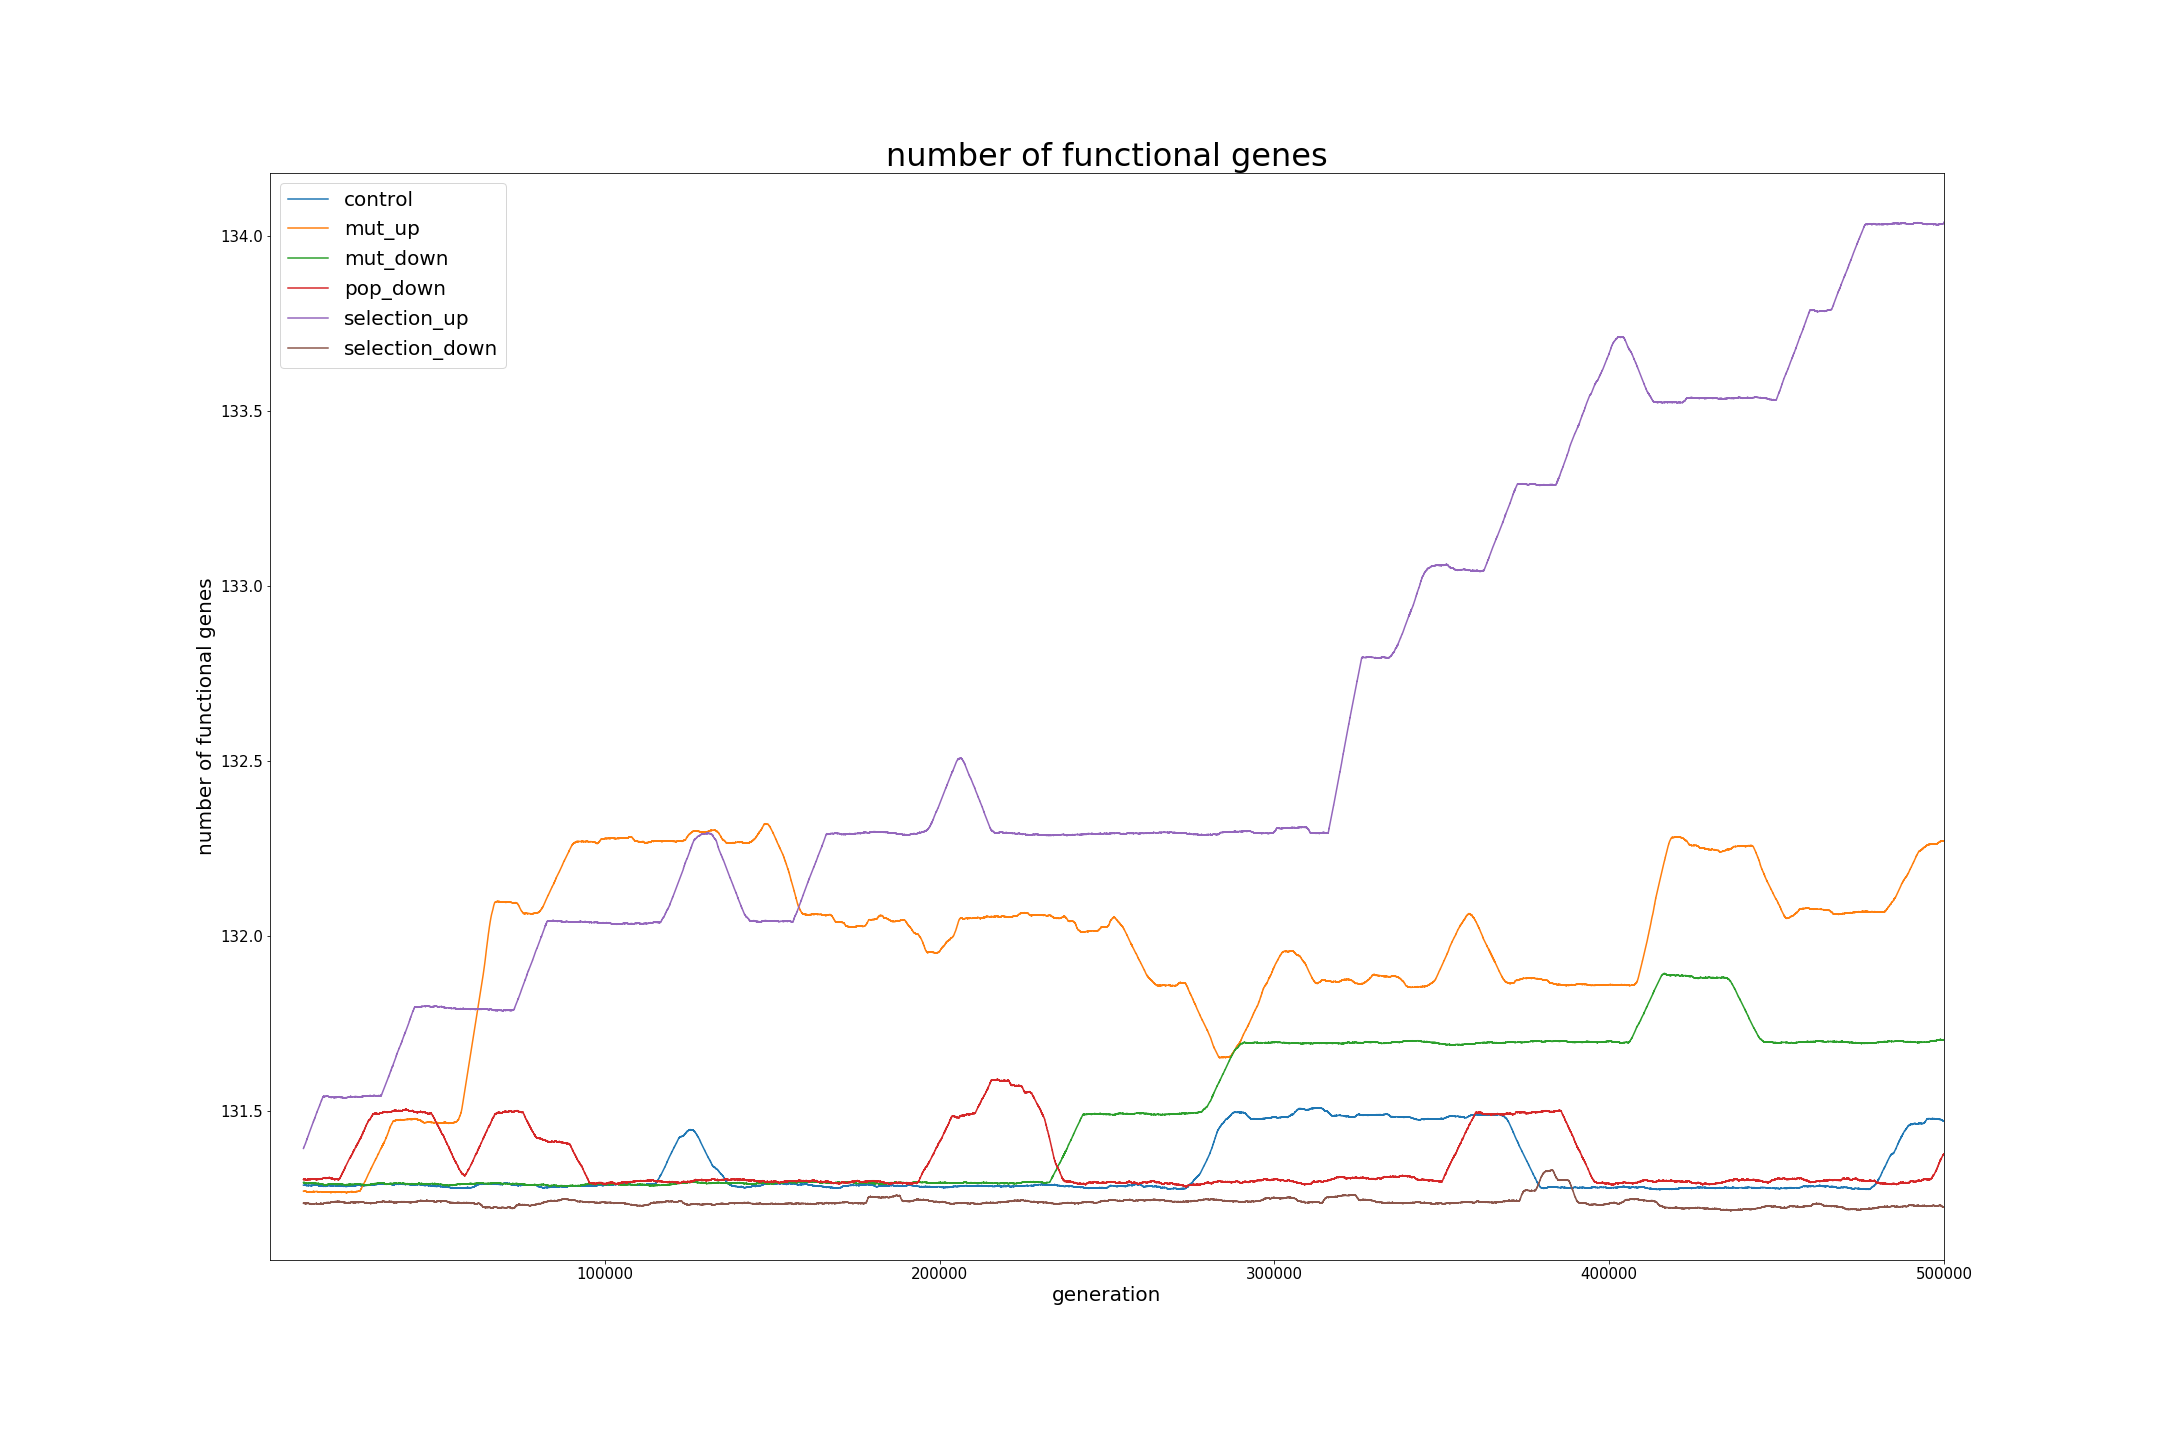
\includegraphics[width=\linewidth]{stat_genes_global_mean_num_functional_genes}
	\caption[Mean number of functional genes]{Plot showing the mean number of functional genes over time across all seeds.}
	\label{fig:mean_num_functional_genes}
\end{figure}
As seen in the figure, the \textit{selection up} condition showed the greatest increase in the number of functional genes in the whole population, reaching a maximum increase of about 2.2\% (131 to 134). This is in agreement with our predictions (from Table~\ref{table:experiment_predictions}) and the findings of Knibbe et al.~\cite{Knibbe2007}. Whereas most of the other curves are fairly flat, the mutation up condition fluctuates relatively rapidly, owing to the quick increase and decrease in the number of base pairs. 

The mean and standard deviation of each condition is given in Table~\ref{table:number_of_genes_mean_std_dev} below.

\begin{table}[H]
	\centering
	\begin{tabular}{|c|c|c|}
		\hline
		\multicolumn{3}{c}{\Large \textbf{Number of Functional Genes}} \\
		\hline
		& \textbf{mean} & \textbf{standard deviation} \\
		\hline
		Control & 131.33289822159796 & 0.08150846235734634 \\
		\hline
		$\mu_+$ & 131.97477775907822 & 0.25246331309927117 \\
		\hline
		$\mu_-$ & 131.50054072148615 & 0.20757038951512172 \\
		\hline
		$k_+$ & 132.60656804679095 & 0.7195302117186394 \\ 
		\hline
		$k_-$ & 131.2389093250132 & 0.013973734803973407 \\
		\hline
		$N_+$ & & \\
		\hline
		$N_-$ & 131.35051857775917 & 0.08328014006877373 \\
		\hline
	\end{tabular}
	\caption[Number of functional genes - mean and standard deviation]{The mean and standard deviation for the number of functional genes across all seeds and for all conditions.}
	\label{table:number_of_genes_mean_std_dev}
\end{table}
\subsubsection{Number of Non-Functional Genes}
The average number of non-functional genes across all seeds for each condition is illustrated in Figure~\ref{fig:mean_num_non-functional_genes} below, and Table~\ref{table:non-functional_genes_mean_std_dev} provides the mean and standard deviation for all seeds and all conditions.  

\begin{figure}[H]
	\centering
	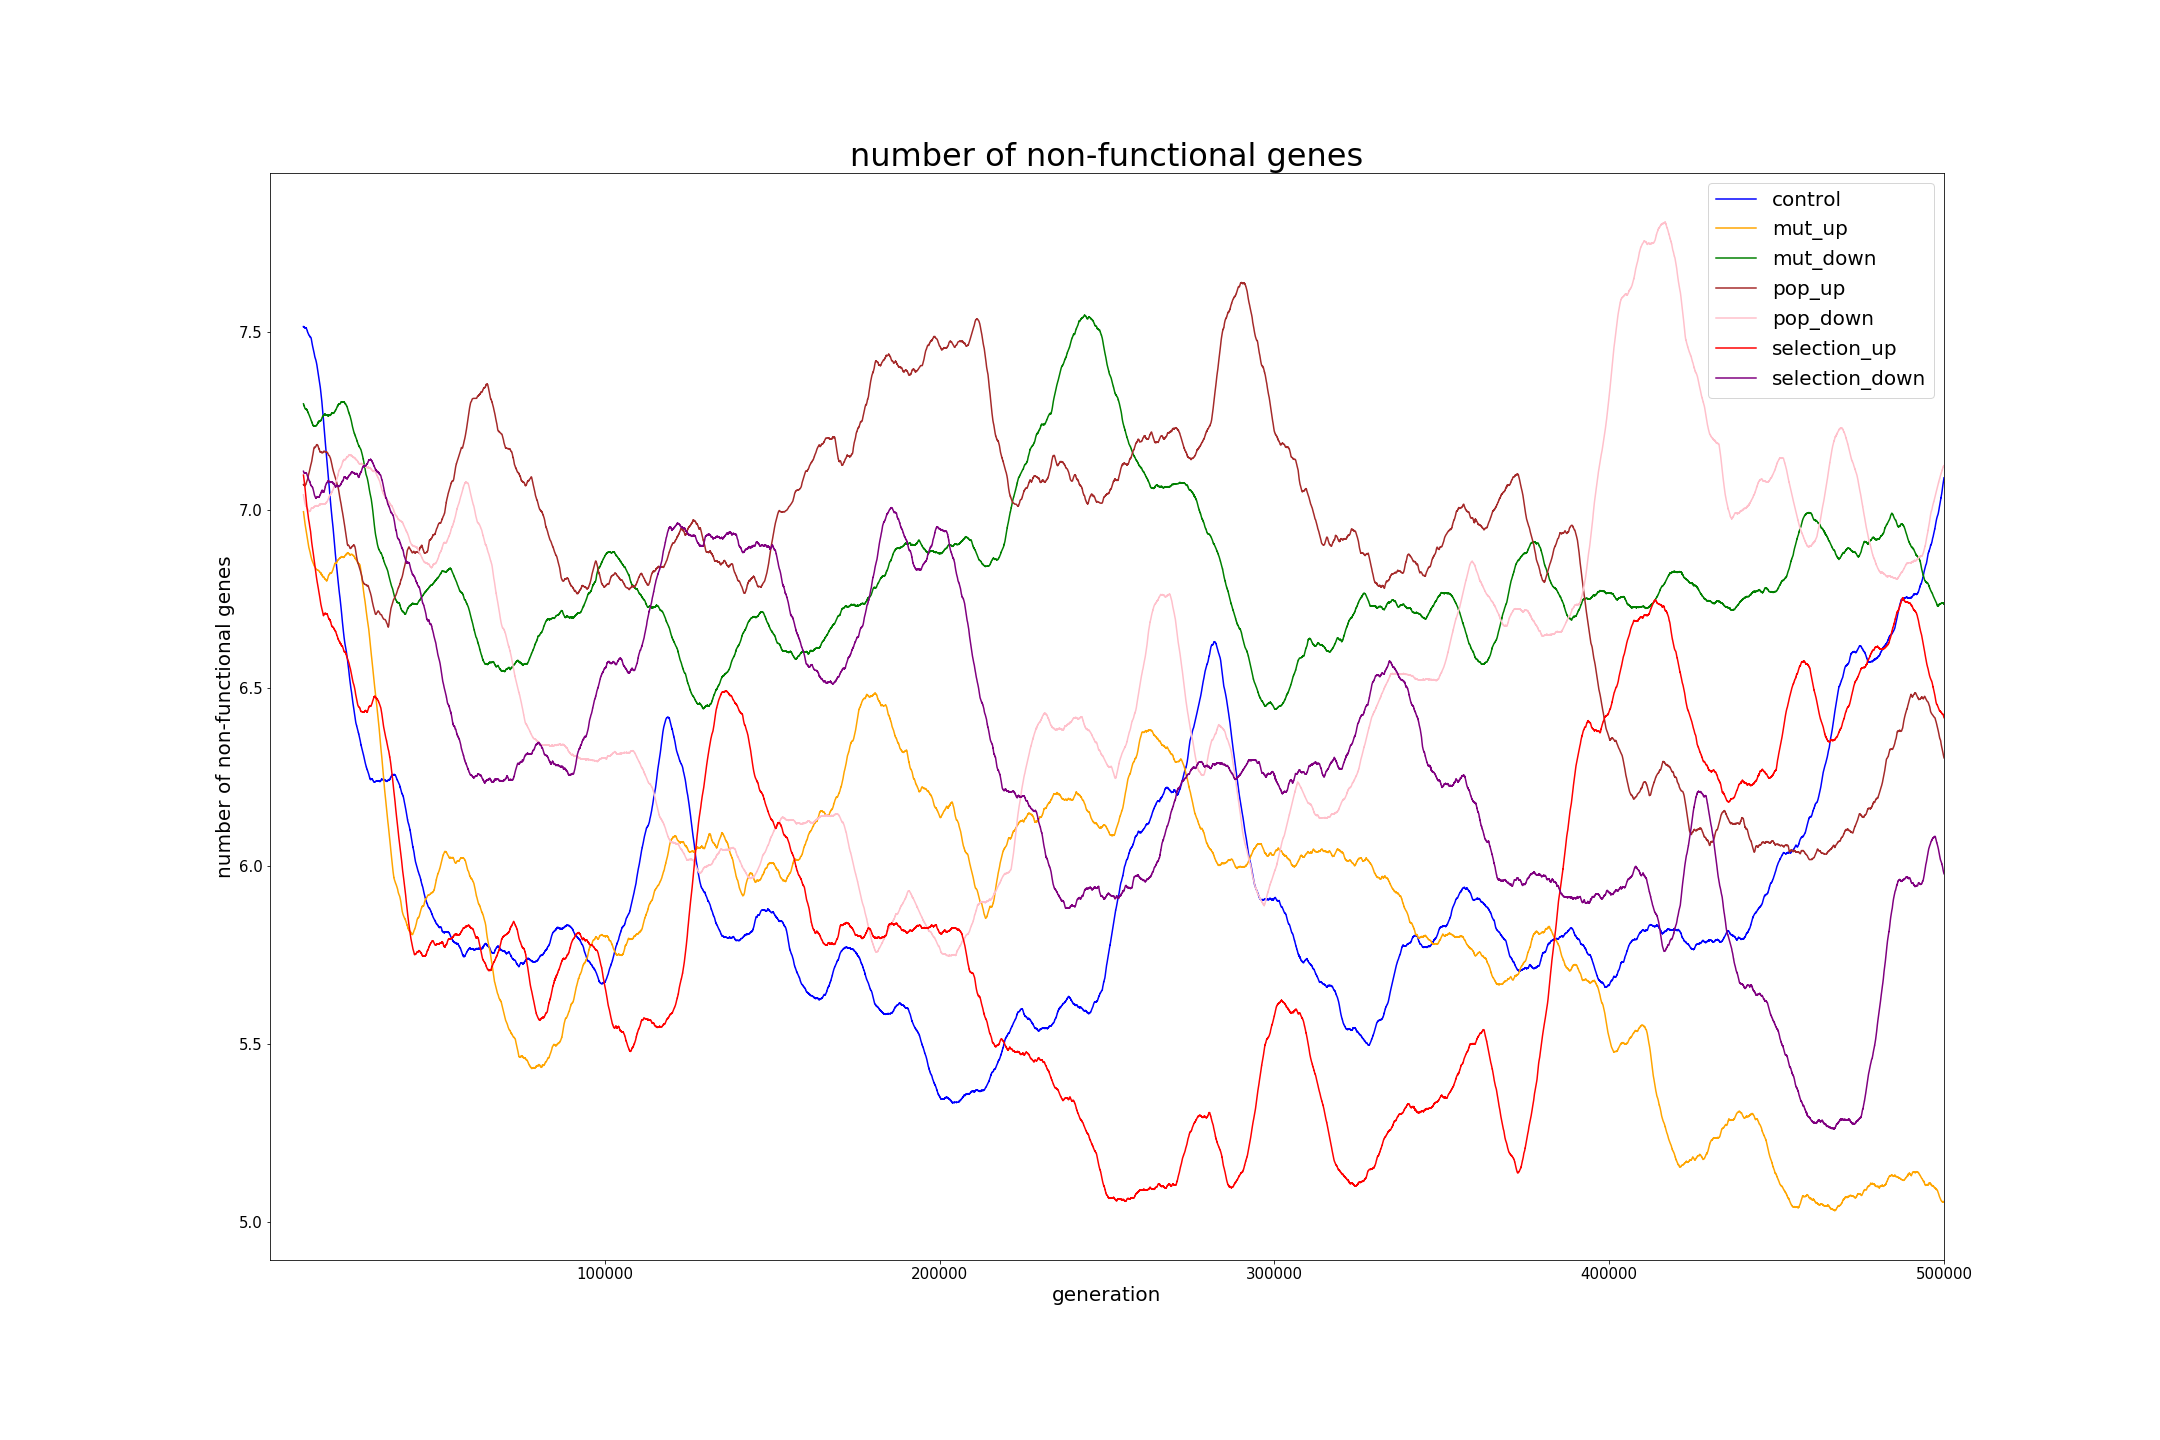
\includegraphics[width=\linewidth]{stat_genes_global_mean_num_non-functional_genes}
	\caption[Mean number of non-functional genes]{The mean number of non-functional genes across all seeds for each condition.}
	\label{fig:mean_num_non-functional_genes}
\end{figure}


\begin{table}[h]
	\centering
	\begin{tabular}{|c|c|c|}
		\hline
		\multicolumn{3}{c}{\Large \textbf{Number of Non-Functional Genes - Mean \& Std. Dev.}} \\
		\hline
		& \textbf{mean} & \textbf{standard deviation} \\
		\hline
		Control & 5.927067481209257 & 0.3857900832994517 \\
		\hline
		$\mu_+$ & 5.856448948104222	& 0.42847313257452385 \\
		\hline
		$\mu_-$ & 6.821347895210327 & 0.22159072539984662 \\
		\hline
		$k_+$ & 5.844289488031533 & 0.5069222102358901 \\
		\hline
		$k_-$ & 6.297804225025876 & 0.45415175059248414 \\
		\hline
		$N_+$ & & \\
		\hline
		$N_-$ & 6.555471025284081 & 0.4836308269184799 \\
		\hline
	\end{tabular}
	\caption[Number of Non-functional Genes - Mean \& St. Dev.]{The mean and standard deviation for the number of non-functional genes, all seeds, all conditions.}
	\label{table:non-functional_genes_mean_std_dev}
\end{table}

\subsubsection{Average Size of Functional Genes}\label{sec:average_size_functional_genes}
Figure~\ref{fig:mean_functional_gene_size} shows the average number of base pairs for each functional gene for the best individual, mapped out over the 500,000 generations. The population down condition continues to be the outlier in terms of genome structure, with the average size of the functional genes remaining noticeably lower than for any other condition. It is worth pointing out, however, that the difference between the smallest average and the largest average is only 1 base pair. 
\begin{figure}[H]
	\centering
	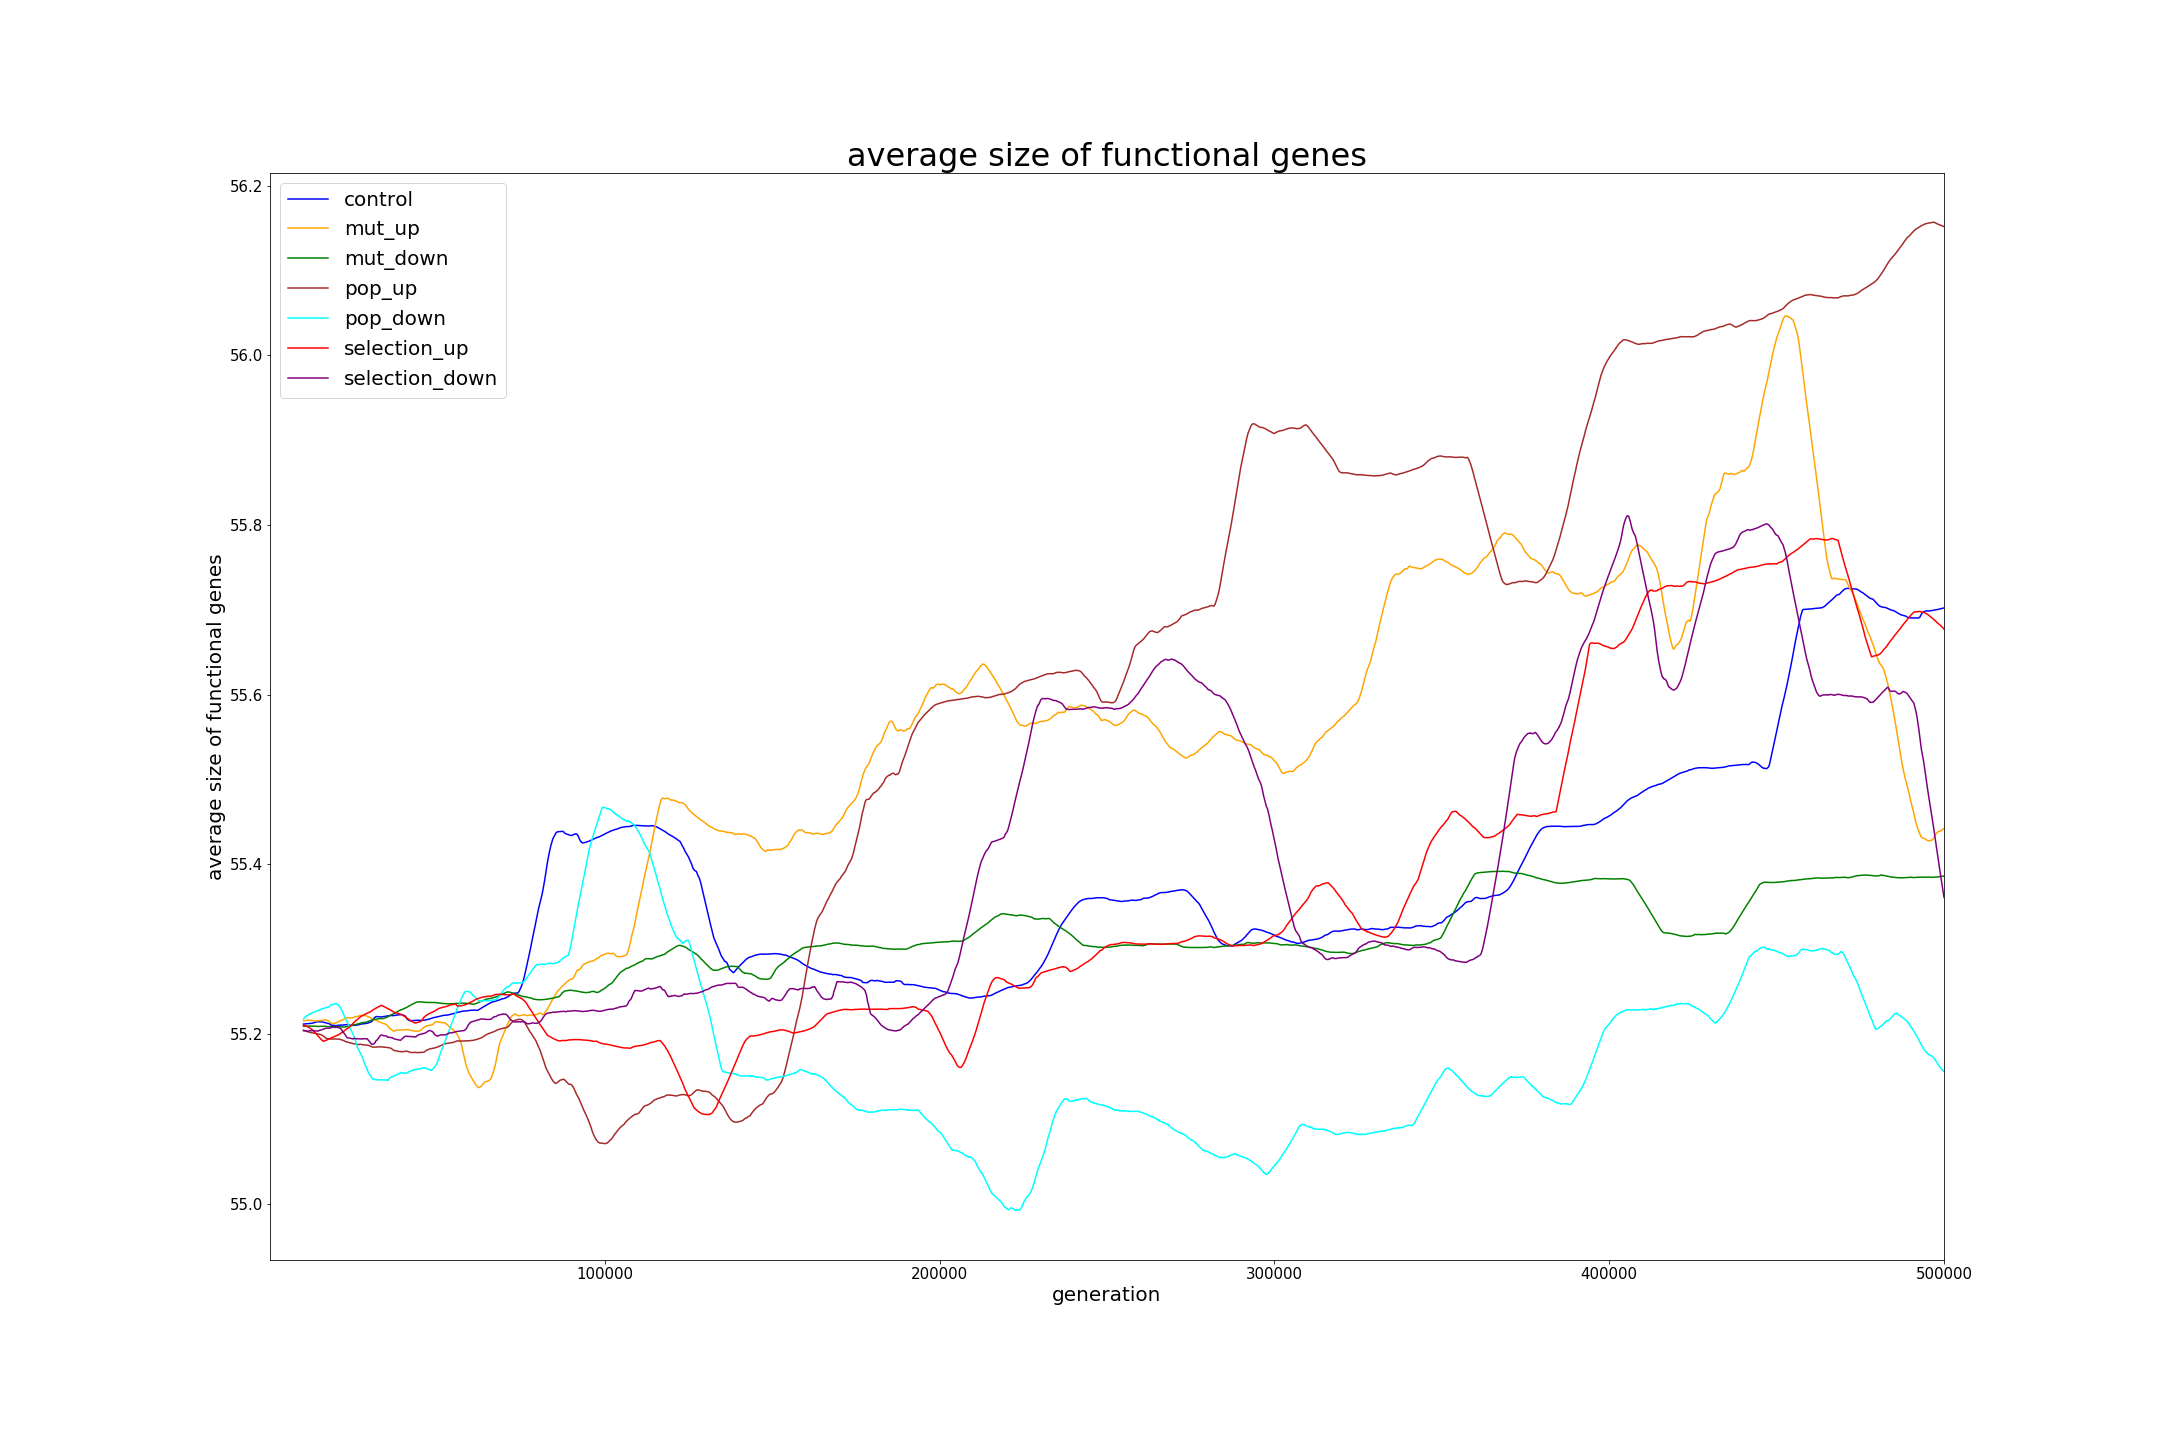
\includegraphics[width=\linewidth]{stat_genes_global_mean_avg_size_of_functional_genes}
	\caption[Average size of functional genes]{Plot showing the average size of functional genes over time for all seeds.}
	\label{fig:mean_functional_gene_size}
\end{figure}
Table~\ref{table:mean_functional_gene_size_and_std_dev} below gives the mean and standard deviation of the results, and Table~\ref{table:avg_size_of_functional_genes_rank_sum_and_p-value} gives the p-values for comparing the control condition to every other condition. 

\begin{table}[H]
	\centering
	\begin{tabular}{|c|c|c|}
		\hline
		\multicolumn{3}{c}{\Large \textbf{Average size of functional genes}} \\
		\hline
		& \textbf{mean} & \textbf{standard deviation} \\
		\hline
		Control & 55.375429751247275 & 0.13745740540215895 \\
		\hline
		$\mu_+$ & 55.5426245000319 & 0.20716437222446815\\ 
		\hline
		$\mu_-$ & 55.309915451000805 & 0.05059383390579744 \\
		\hline
		$k_+$ & 55.37046527382346 & 0.2024427915314053 \\
		\hline
		$k_-$ & 55.414464890880595 & 0.1954246818788886 \\
		\hline
		$N_-$ & 55.17428963311534	& 0.09886004440916518 \\
		\hline
	\end{tabular}
	\caption[Mean functional gene size and standard deviation]{Mean functional gene size and standard deviation, all seeds, all conditions.}
	\label{table:mean_functional_gene_size_and_std_dev}
\end{table}

\begin{table}[H]
	\begin{tabular}{|c|c|c|}
		\hline
		\multicolumn{3}{c}{\Large \textbf{Average size of functional genes - rank sum \& p-value}} \\
		\hline
		& \textbf{rank sum} & \textbf{p-value} \\
		\hline
		$\mu_+$ & 68252491056.0 & 0.00000000000000 \\
		\hline
		$\mu_-$ & 96067062201.5 & 0.00000000000000 \\
		\hline
		$N_-$ & 28963878467.0 & 0.00000000000000 \\
		\hline
		$k_+$ & 103481641646.0 & 0.00000000000000 \\
		\hline
		$k_-$ & 124890321462.0 & 0.223664707704009 \\
		\hline
	\end{tabular}
	\caption[Average size of functional genes - rank sum and p-value]{Average size of functional genes - rank sum and p-value for all conditions and all seeds.}
	\label{table:avg_size_of_functional_genes_rank_sum_and_p-value}
\end{table}
Since the $k_-$ condition's p-value was $\geq0.05$, we must conclude that these results are not significant. 

\subsection{Evolvability}
In Figure~\ref{fig:evolvability_mean} below, we see the results of the experiments on evolvability for the best individual's (at generation 500,000) lineage. 
\begin{figure}[H]
	\centering
	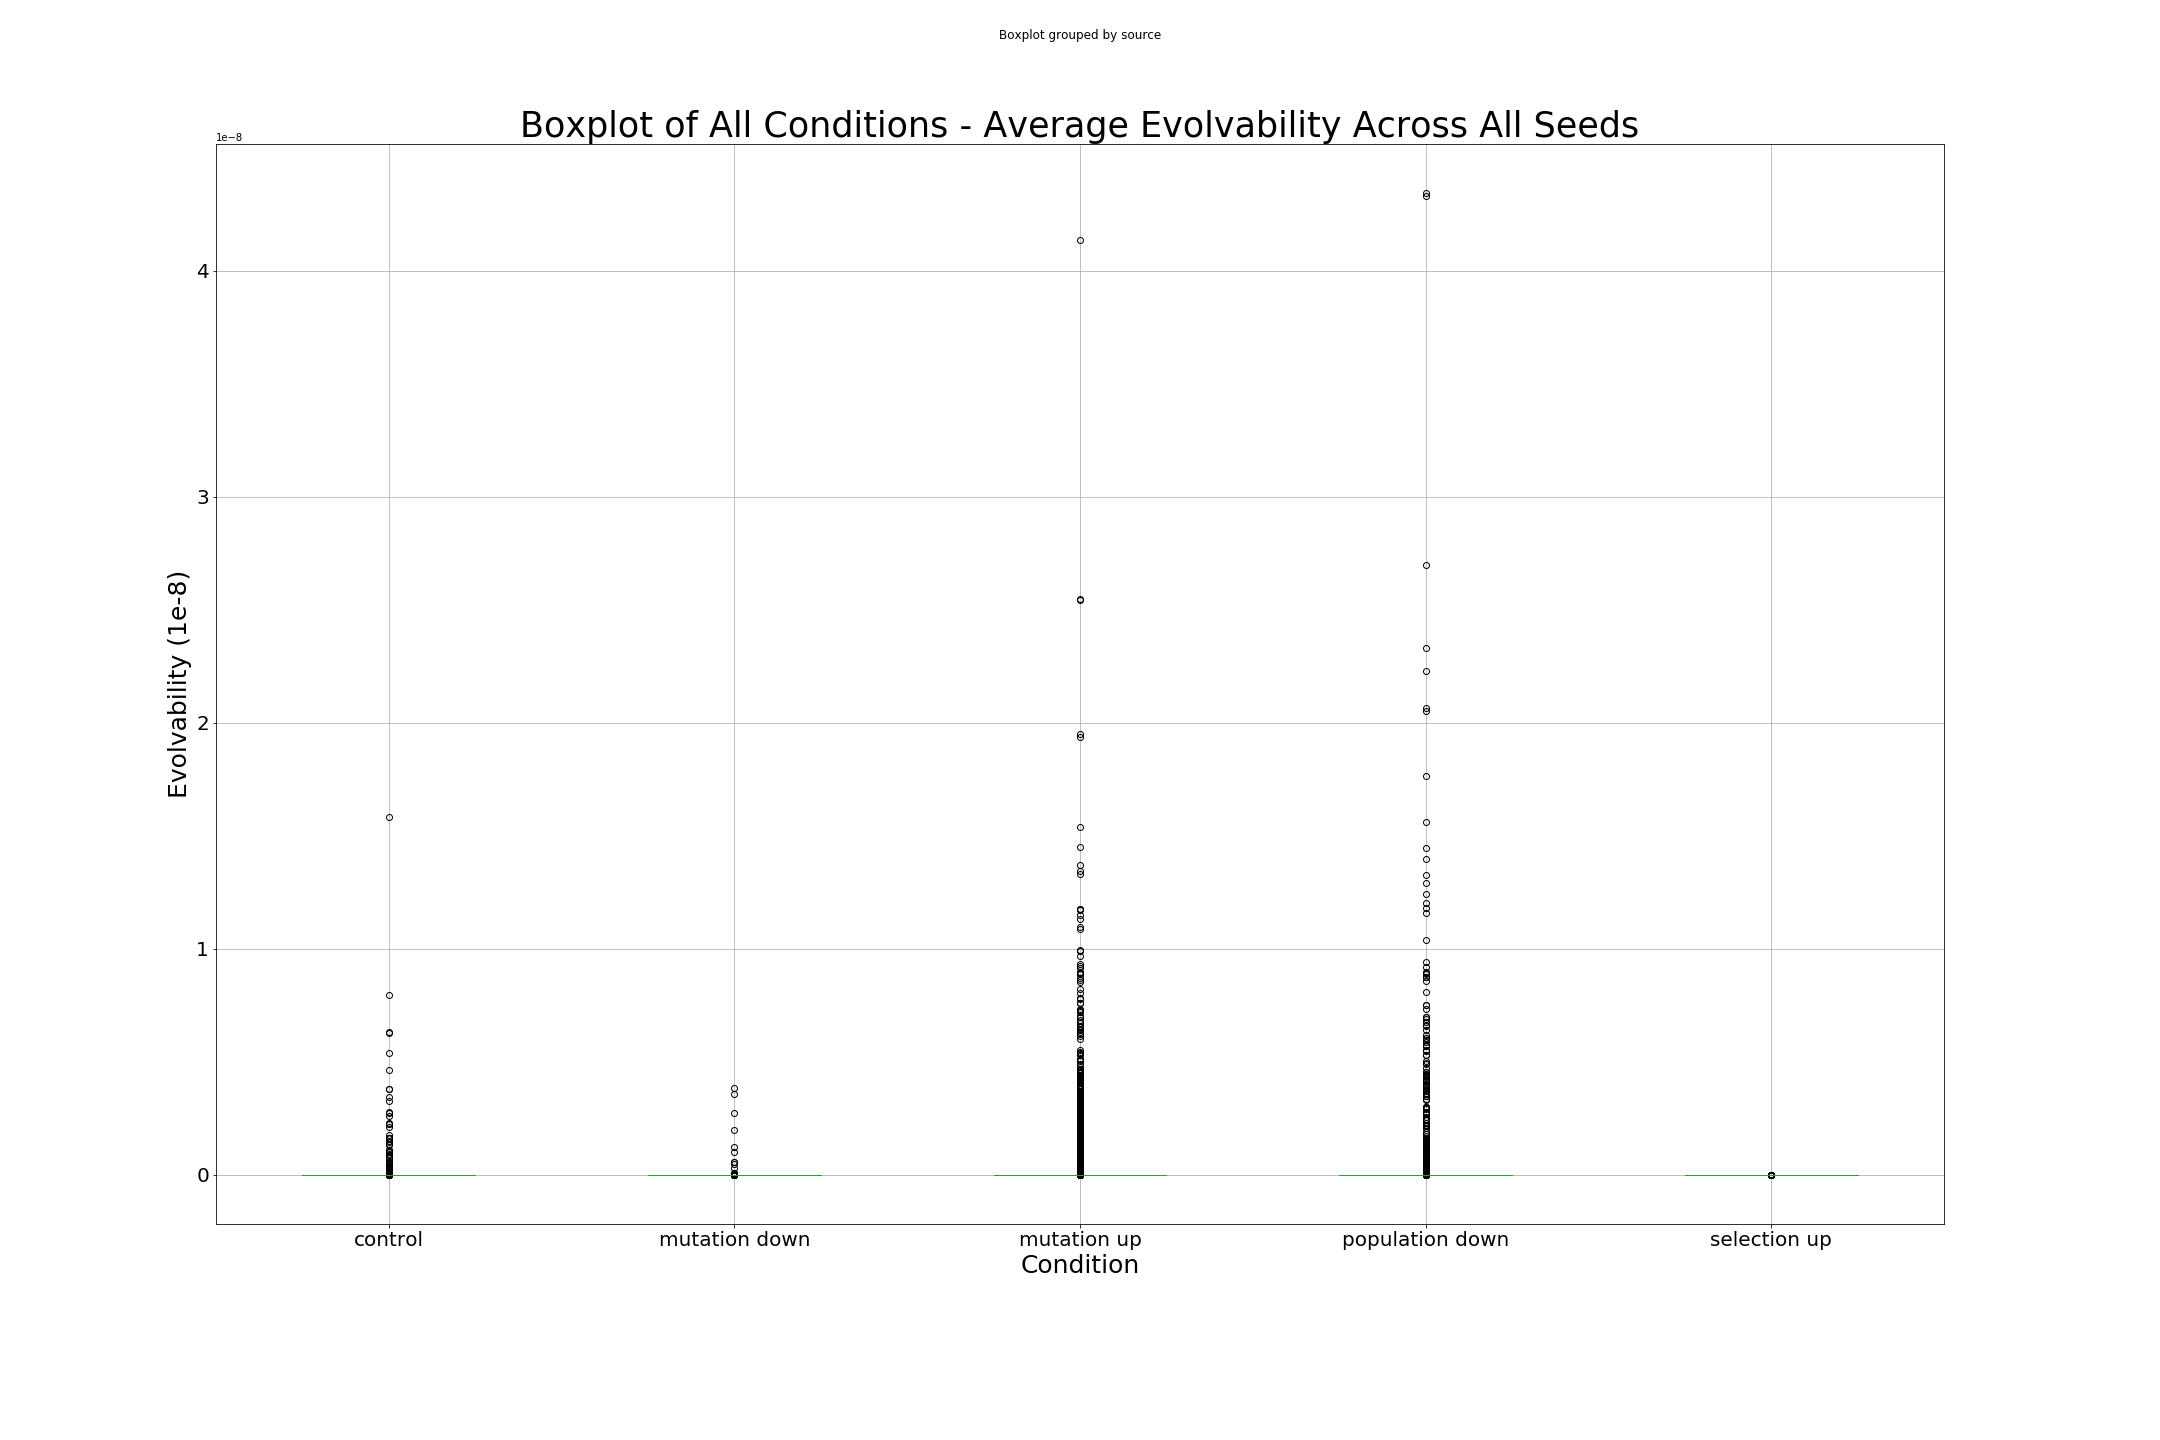
\includegraphics[width=\linewidth]{evolvability_boxplot_all_seeds_avg}
	\caption[Evolvability boxplot]{A box plot showing the mean evolvability spread of all seeds and all conditions. Higher numbers are more evolvable.}
	\label{fig:evolvability_mean}	
\end{figure}
The figure illustrates that, for each condition, overall the best individual still had quite low evolvability. For the selection up condition, however, the deviation from zero was even smaller, as illustrated in Table~\ref{table:mean_std_dev_evolvability} below, which provides the mean and standard deviation of the evolvability of the best individual in each condition. 

The evolvability rank sum and p-value information is given in Table~\ref{table:evolvability-rank_sum_and_p-values}.

\begin{table}[H]
	\begin{tabular}{|c|c|c|}
		\hline
		\multicolumn{3}{c}{\Large \textbf{Evolvability rank sum and p-value}} \\
		\hline
		& \textbf{rank sum} & \textbf{p-value} \\
		\hline
		$\mu_+$ & 36203620.0 & 0.000000000309416 \\
		\hline
		$\mu_-$ & 7025283.5 & 0.010212448990316 \\
		\hline
		$k_+$ & 13181851.5 & 0.000000000000074 \\
		\hline
		$k_-$ & 13779001.5 & 0.000000084666842 \\
		\hline
		$N_+$ & & \\
		\hline
		$N_-$ & 19403134.5 & 0.00000000000000 \\
		\hline
	\end{tabular}
	\caption[Evolvability - rank sum and p-value]{Rank sum and p-values for evolvability, all seeds, all conditions.}
	\label{table:evolvability-rank_sum_and_p-values}
\end{table}

\begin{table}[H]
	\centering
	\begin{tabular}{| c | c | c |}
		\hline
		\multicolumn{3}{c}{\Large Evolvability - Mean \& Std. Dev.} \\
		\hline
		& \textbf{mean} & \textbf{standard deviation}\\
		\hline
		\hline
		control & 2.035523813975702e-11 & 3.2787490312081233e-10\\
		\hline
		$\mu_+$ & 9.97655150597127e-11 & 8.41749150634588e-10 \\
		\hline
		$\mu_-$ & 6.064697990806935e-12 & 1.2471674281540128e-10 \\
		\hline
		$k_+$ & 1.9498939718794653e-15 & 6.394659146405824e-14 \\
		\hline
		$k_-$ & 4.3065723639721706e-10 & 5.20232907351617e-09 \\
		\hline
		%TODO Fill in population up
		$N_+$ &  & \\
		\hline
		$N_-$ & 8.837632116681012e-11 &  1.0799303682398726e-09 \\
		\hline	 		 
	\end{tabular}
	\caption[Evolvability mean and standard deviation]{Table illustrating the mean and standard deviation of the evolvability for each condition. $\mu$ is the mutation rate, $k$ is the selection rate, and $N$ is the population size.}
	\label{table:mean_std_dev_evolvability}
\end{table}

\subsection{Robustness}
Recall from Section~\ref{subsec:robustness_antirobustness} that robustness is measured by the fraction of neutral offspring of an individual. In the following figure, we see a bar plot showing the spread of neutral offspring for the best individual for the control condition as well as the six variations. 

%TODO update graphic with more conditions once experiments are completed
\begin{figure}[H]
	\centering
	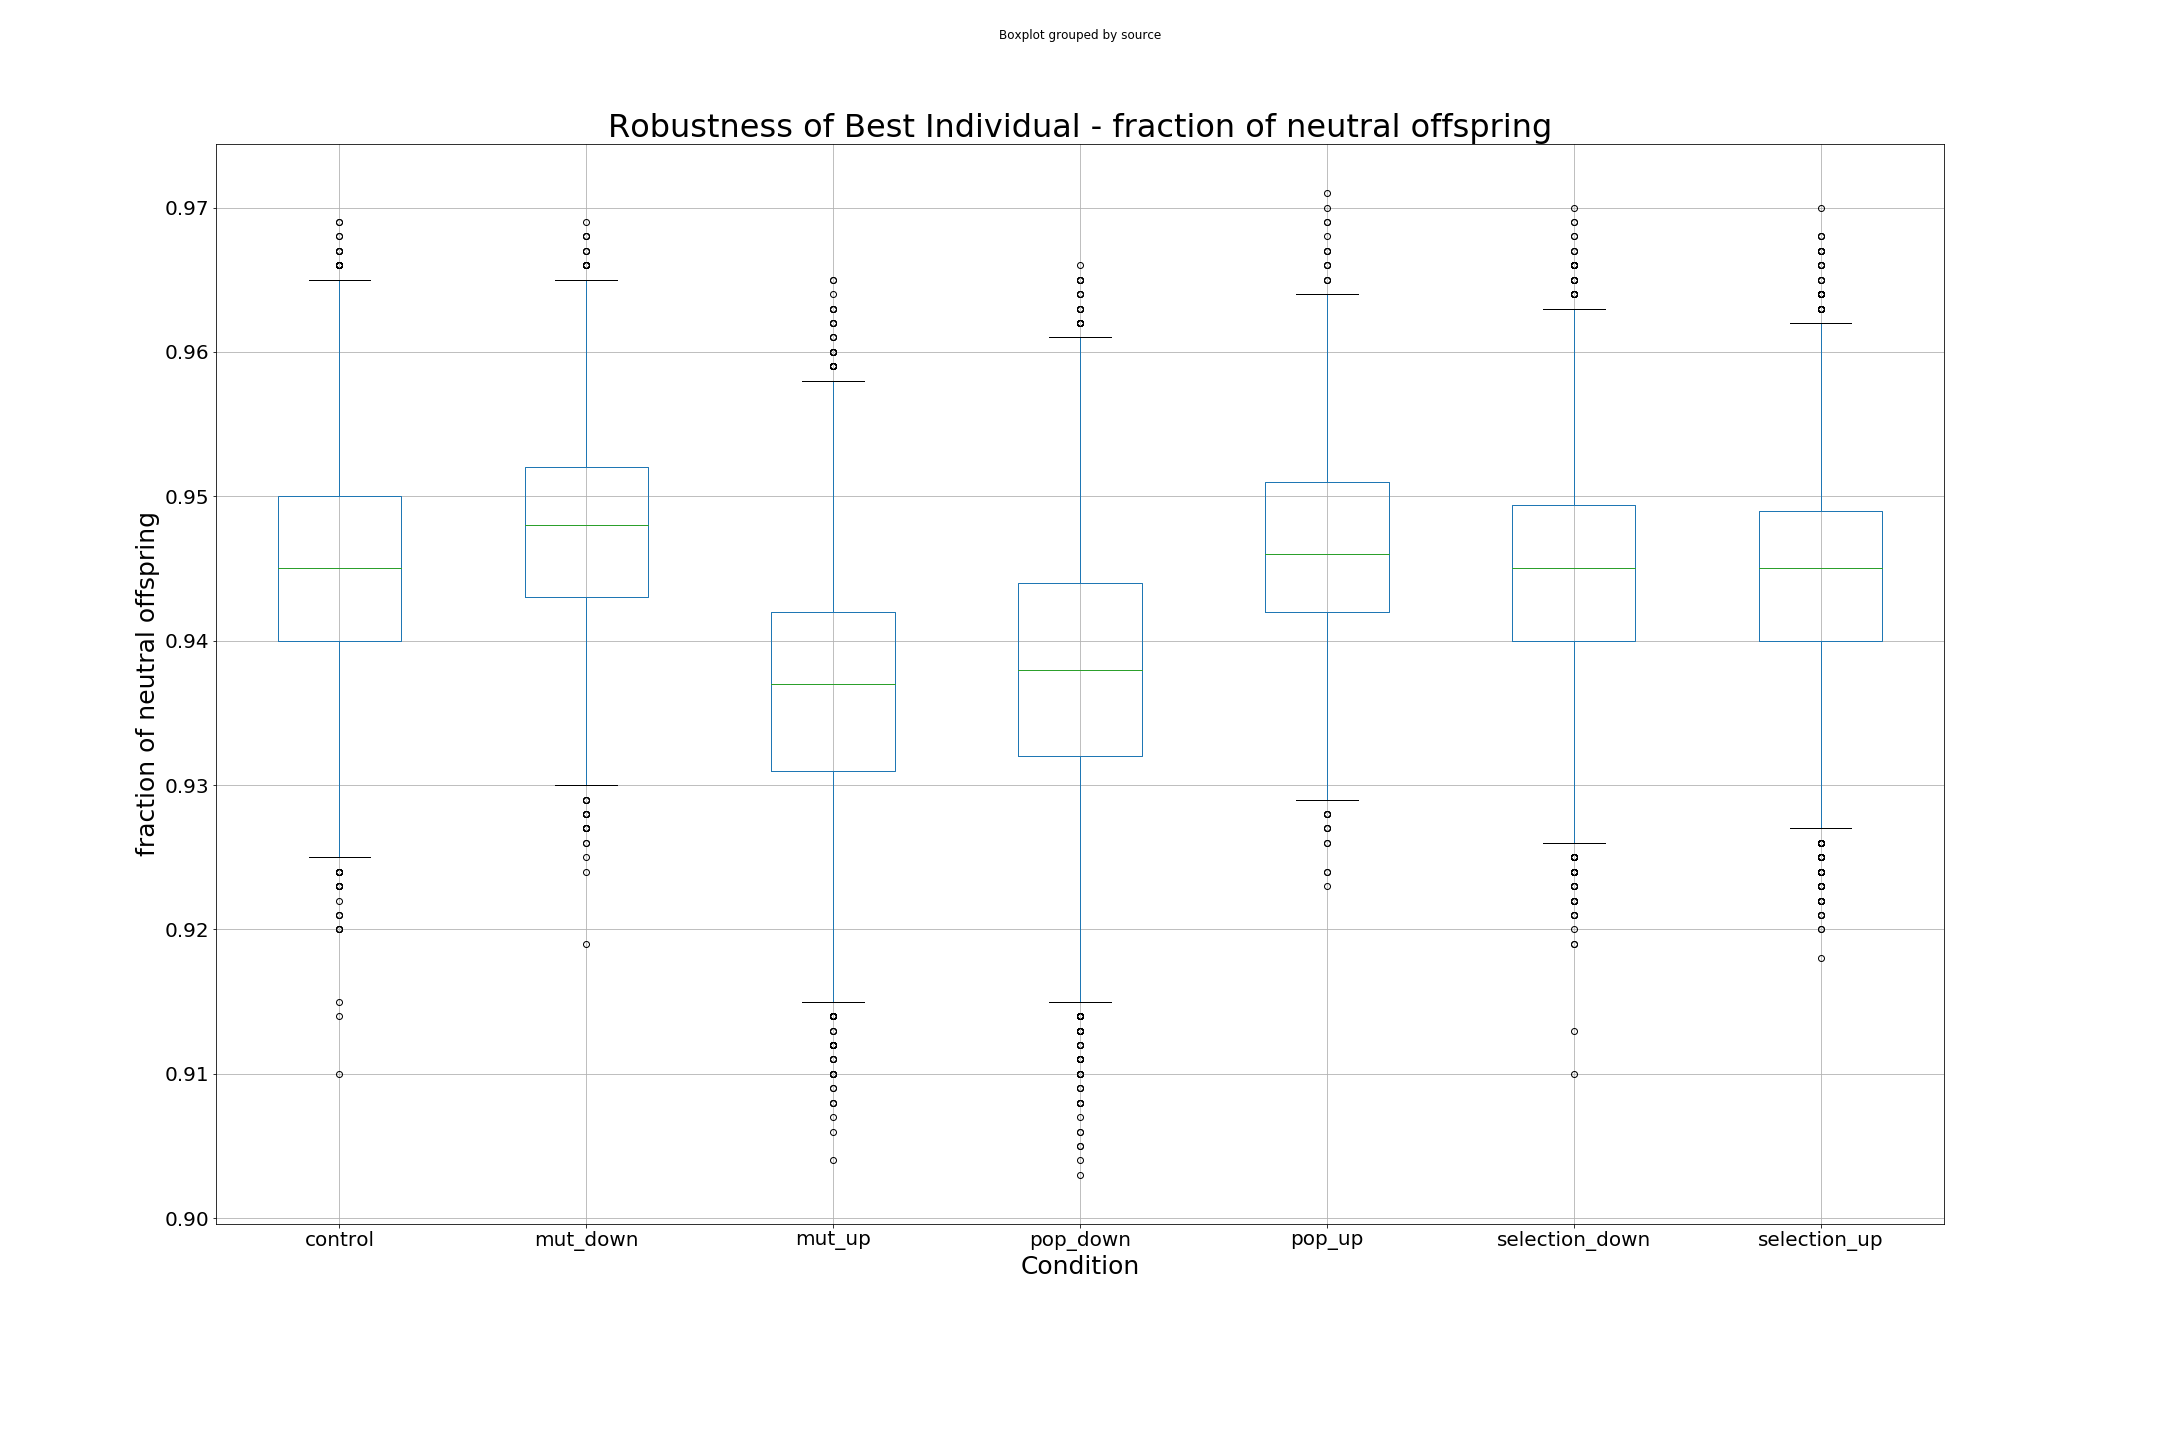
\includegraphics[width=\linewidth]{stat_robustness_best_mean_frac_neutral_offspring}
	\caption[Robustness bar graph]{Bar graph showing the spread of neutral offspring for the best individual at generation 500,000, all conditions.}
	\label{fig:mean_robustness_all_conditions}
\end{figure}
The mutation up condition clearly had the largest mean percentage of neutral mutants, at 0.5\%. The full statistics are given in the tables below:

\begin{table}
	\begin{tabular}{|c|c|c|}
		\hline
		\multicolumn{3}{c}{\Large \textbf{Robustness - Rank Sum \& p-values}} \\
		\hline
		& \textbf{rank sum} & \textbf{p-value} \\
		\hline
		$\mu_+$ & 16756710.5 & 0.000000000000000 \\
		\hline
		$\mu_-$ & 5741758.0 & 0.000000000000000 \\
		\hline
		$N_-$ & 12493750.0 & 0.000000000000000 \\
		\hline
		$k_+$ & 13580845.5 & 0.001358704915202 \\
		\hline
		$k_-$ & 13925884.0 & 0.001273247024315 \\
		\hline
	\end{tabular}
	\caption[Robustness rank sum \& p-values]{Mean robustness rank sum and p-values for all conditions and all seeds.}
	\label{table:rank_sum_p-values}
\end{table}
\begin{table}[H]
	\begin{tabular}{|c|c|c|}
		\hline
		\multicolumn{3}{c}{\Large \textbf{Robustness - means \& standard deviations}} \\
		\hline
		& \textbf{rank sum} & \textbf{p-value} \\
		\hline
		Control & 0.944925327538429	& 0.007334383035973237 \\
		\hline
		$\mu_+$ & 0.9366773604226319 & 0.007907308763606846 \\
		\hline
		$\mu_-$ &	0.94754266274366 & 0.0070662676155014035 \\
		\hline
		$k_+$ & 0.9444661080775791 & 0.007371509508882273 \\
		\hline
		$k_-$ & 0.9445156995960435	& 0.007423851661757711 \\
		\hline
		$N_-$ & 0.9374093190746451 & 0.008846010304259707 \\
		\hline
	\end{tabular}
	\caption[Robustness means and standard deviations]{Robustness means and standard deviations for all conditions and all seeds.}
	\label{table:robustness_means_and_std_dev}
\end{table}


\section{Discussion}\label{discussion}

Analogously to Table~\ref{table:experiment_predictions}, we summarize the results of our experiments in Table~\ref{table:experiment_results_summary} below. For each cell, {\color{green} green} indicates that our prediction was confirmed in our experiments and {\color{red}red} indicates that the prediction must be rejected. Our predictions for each condition are duplicated here for convenience, with a $+$ indicating a predicted increase and $-$ indicating a predicted decrease over the control condition. 

%TODO Is this table from Chapter 3 correct? Specifically, is mutation+/- right for fitness? 
\begin{table}[H]
	\centering
	\begin{tabular}{|c||c|c|c|c|c|c|}
		\hline
		\multicolumn{7}{|c|}{{\Large \textbf{Experiment Results Summary}}} \\
		\hline \hline
		\multirow{2}{*}{\textbf{Effect On:}} & \multicolumn{6}{c|}{\textbf{Condition}} \\
		\cline{2-7}
		& {\Large$\mu_+$} & {\Large$\mu_-$} & {\Large$k_+$} & {\Large$k_-$} & {\Large$N_+$} & {\Large$N_-$} \\
		\hline 
		Genome Size & \cellcolor{green} $-^{\cite{bradwell2013correlation, marais2008mutation}}$ & \cellcolor{red} $\text{+}^{\cite{bradwell2013correlation, drake1991constant}}$ & \cellcolor{green} $+^{\cite{Batut.2013}}$ & \cellcolor{green} $-^{\cite{Batut.2013}}$ & $-^{\cite{Batut.2014}}$ & \cellcolor{green} $+^{\cite{Batut.2014}}$ \\
		\hline
		Fitness & \cellcolor{green} $+^{\cite{bataillon2000estimation, vahdati2017effect}}$ & \cellcolor{green} $-^{\cite{vahdati2017effect}}$ & \cellcolor{red} $+^{\cite{Batut.2014}}$ & \cellcolor{red} $-^{\cite{Batut.2014}}$ & $+^{\cite{cutter2019primer, vahdati2017effect}} $ & \cellcolor{green} $-^{\cite{cutter2019primer, vahdati2017effect}} $\\
		\hline
		Amount of non-coding DNA & \cellcolor{green} $-^{\cite{Knibbe2007}}$ & \cellcolor{red} $+^{\cite{Knibbe2007}}$ & \cellcolor{green} $+^{\cite{Batut.2013, Knibbe2007}}$ & \cellcolor{green} $-^{\cite{Batut.2013, Knibbe2007}}$ & $-^{\cite{Batut.2013}}$ & \cellcolor{green} $+^{\cite{Batut.2013}}$ \\
		\hline
		Number of genes & \cellcolor{red} $-^{\cite{Knibbe2007}}$ & \cellcolor{green} $+^{\cite{Knibbe2007}}$ &\cellcolor{green} $+^{\cite{Knibbe2007}}$ & \cellcolor{green} $-^{\cite{Knibbe2007}}$ & $-^{\cite{Batut.2014}}$ & \cellcolor{green} $+^{\cite{Batut.2014}}$ \\
		\hline
		Average size of genes & \cellcolor{red} $-^{\cite{Liard.2018}}$ & \cellcolor{green} $+^{\cite{Liard.2018}}$ & \cellcolor{green} $-^{\cite{Batut.2013}}$ & \cellcolor{red}$+^{\cite{Batut.2013}}$ & $-^{\cite{Batut.2014}}$ & \cellcolor{red} $+^{\cite{Batut.2014}}$ \\
		\hline
		Robustness & \cellcolor{green} $-^{\cite{Knibbe2007}}$ &\cellcolor{green} $+^{\cite{Knibbe2007}}$ & \cellcolor{green} $-^{\cite{Batut.2013, Knibbe2007}}$ & \cellcolor{green}$+^{\cite{Batut.2013, Knibbe2007}}$ & $-^{\cite{elena2007effects}}$ & \cellcolor{red} $+^{\cite{elena2007effects}}$ \\
		\hline
		Evolvability &\cellcolor{green} $+^{\cite{Knibbe2007}}$ &\cellcolor{green} $-^{\cite{Knibbe2007}}$ & \cellcolor{red}  $+^{\cite{Batut.2013}}$ & \cellcolor{red} $-^{\cite{Batut.2013}}$ & $-^{\cite{wein2019effect}}$ & \cellcolor{green} $+^{\cite{wein2019effect}}$ \\
		\hline		
	\end{tabular}
	\caption[Experiment result summary]{A summary of whether our experiment results confirmed or denied the hypotheses of Table~\ref{table:experiment_predictions}.  were confirmed ({\color{green}green}) or rejected ({\color{red}red}), along with the predicted results of whether the given result would increase (+) or decrease (-) over the control condition.}
	\label{table:experiment_results_summary}
\end{table}

According to our predictions based on a survey of the literature (summarized in Table~\ref{table:experiment_predictions}), the $\mu_+$, $k_-$, and $N_+$ conditions should have lead to a reduced genome. As shown in Figure~\ref{fig:genome_size} however, none of these predictions held up, and in fact the genome size increased in all conditions, including those that were predicted to be reduced. One possible explanation is that, because the wild types had already been evolving for 10 million generations, and we did not vary the environment further for our experiments, perhaps they had reached a sort of stasis for which another half-million generations were not sufficient to fully demonstrate the effects of any changes. This may not explain everything, however, as some conditions (e.g. $\mu_+$, $N_-$) did see a rather rapid change in fitness, genome structure, etc. even in the (comparatively) short time. 

Also of interest is that, along with the genome size, overall the fitness of the organisms did not change much with only one exception ($k_+$). It has been postulated that perhaps gene loss may be selected for in order to increase the overall fitness of an organism by removing the added cost of the superfluous genes~\cite{koskiniemi2012}. Our results do not fully agree with this hypothesis, as our results show that, in addition to the general accumulation of non-coding DNA across all conditions (Figure~\ref{fig:mean_non-coding_DNA}), which would theoretically have a higher fitness cost, the number of genes actually \textit{increased} slightly for each condition, except for $k_-$. Likewise, fitness overall went \textit{up} as the number of genes increased (except for $N_-$). Lastly, decreasing the selection pressure resulted in the highest overall mean fitness by a wide margin (Table~\ref{table:fitness_means_std_dev}). In Aevol, non-coding DNA is not really associated with a fitness cost, so this explanation may likely also not fully apply. 

Regarding the $N_-$ condition, comparing this with the results of Batut et al. and their work with \textit{Buchnera aphidicola} (see Section~\ref{related_work}), it may be possible that gene loss is occurring because of the smaller effective population size clicking down Muller's Ratchet. This does not seem to be what is happening in our experiments either, however. Though mean fitness of the $N_-$ condition did greatly decline (see Figure~\ref{fig:mean_fitness_plot}), the $N_-$ condition also saw the largest accumulation of non-coding DNA (see Figure~\ref{fig:mean_non-coding_DNA}) and the second-highest level of evolvability (see Table~\ref{table:mean_std_dev_evolvability}), which should theoretically have lead to an easier time of overcoming the ratchet. On the other hand, the number of functional genes stayed more or less the same as all of the other conditions, and the accumulated number of non-functional genes (pseudogenes) of the $N_-$ condition was the largest (see Figure~\ref{fig:mean_num_non-functional_genes}). These two factors together suggest that there almost certainly was some loss of fitness through pseudogenization; perhaps with more time, the pseudogenes would also have been lost.

Recall the work of Liard et al.\cite{Liard.2018} as discussed in Section~\ref{related_work}, in which the proposed ``complexity ratchet'' was overcome by increasing the mutation rate. Their work was quite successful in overcoming this ratchet, but in our experiments, both the number of genes and the average size of the genes increased. One possible explanation for this is that, in their work, their increased mutation rate $\mu_+$ was set to $1e^{-3}$.  By contrast, even our elevated mutation rate, $\mu_+$, was just $4e^{-7}$, which is $\frac{1}{4}*e^4 \approx 13.65$ times lower than their highest mutation rate. Perhaps an even higher mutation rate would be sufficient to overcome the power of selection and reduce the genome further. 

%TODO Perform another experiment with a much higher mutation rate: 1e-3 for 100k generations?



\chapter{Conclusions and Future Work}\label{ch:conclusion}
In this section we will summarize our overall conclusions drawn from the work, discuss some limitations of our experiments, and highlight a few possibilities for further research.

\section{Conclusions}
Although the mean values for genome size given in Table~\ref{table:genome_size_mean_and_std_dev} suggest that only the $\mu_-$ condition lead to a reduced genome, at generation 500,000 there were three conditions in which the genome size was lower than the control condition (see Figure~\ref{fig:genome_size}): $\mu_+$, $k_-$, and surprisingly $m_-$. 

\section{Relation to Real-World Organisms}
%TODO Complete Section - Relation to Real-World Organisms
We began this thesis with the intention of examining the factors that may drive reductive evolution, with the overall intention of relating this to real-world examples. The marine cyanobacteria \textit{Prochlorococcus} has large effective population sizes and high adaptability, which has resulted in a large number of ecotypes which exist at differing depths in the oligotrophic oceans. 
  
\section{Limitations and Future work}\label{limitations}
%TODO Complete Section - Limitation of Results
\subsection{Parameters}
Although it was the main design of our experiments, one limitation to consider is that only one parameter varied per condition. It may be possible that it is only under a combination of conditions that reductive evolution more reliably occurs. Since both an increased mutation rate and decreased selection pressure lead to a reduced genome in our experiments, it may be worth testing whether a combination of the two would lead to an even greater reduction. 

In a similar vein, we only tested one value for each changed condition. For example, only a mutation rate of $\mu_+ = 4e^{-7}$ was tested for the $\mu_+$ condition. Perhaps an even higher mutation rate, such as $\mu_+ = 1e^{-3}$, might be enough to reduce the number of genes, as predicted by Knibbe et al.~\cite{Knibbe2007} and \cite{Liard.2018}. Their mutation rates were $2.1e^{-5}$ and $1e^{-3}$, roughly $3.9$ and $13.65$ times higher than our rate. The testing of more extreme values for each parameter may provide a fuller picture of the balance between selection, mutation rates, population sizes, and reductive genomes. 

\subsection{Environments}
Another limitation is that the environments did not vary in our experiments. Aevol includes the ability to vary the environment natively, so future experiments could vary the environment over time to see if doing so would increase or decrease robustness or evolvability, which are strong drivers of reductive evolution~\cite{Batut.2013}. 

\subsection{Limitations of the Aevol Model}
Aevol as a modeling software is limited in that, like all models, it relies on several simplifications. For example, the population sizes tested here, even in the population up condition, are still much smaller than would be found in real world populations. It could be that in order to properly judge the effects of Muller's Ratchet under differing conditions, we need much larger population sizes. 

%\input{Chapter6.tex}

\blankpage

% usare questo invece di usare \appendix perchè l'altro dà un ref sbagliato sul primo link dell'indice
\begin{appendices}
	%\chapter{Glossary}
\label{appendixA}
Just comment \verb|\chapter{Glossary}
\label{appendixA}
Just comment \verb|\chapter{Glossary}
\label{appendixA}
Just comment \verb|\input{AppendixA-Glossary.tex}| in Masterthesis.tex if you don't need it!

\begin{longtable}{p{2.5cm}p{9.5cm}}

\huge{\textbf{Symbols}}& \\
\hline
\\
\$ & US. dollars. \\
\\
\\
\huge{\textbf{A}}& \\
\hline
\\
A& Meaning of A.\\
\\
\\
\huge{\textbf{B}}& \\
\hline
\\

\\
\\
\huge{\textbf{C}}& \\
\hline
\\

\\
\\
\huge{\textbf{D}}& \\
\hline
\\

\\
\\
\huge{\textbf{E}}& \\
\hline
\\

\\
\\
\huge{\textbf{F}}& \\
\hline
\\
Fixed mutation rate& The measured mutation rate at the end of the experiments.
\\
\\
\huge{\textbf{G}}& \\
\hline
\\
\\
\\
\huge{\textbf{H}}& \\
\hline
\\

\\
\\
\huge{\textbf{I}}& \\
\hline
\\

\\
\\
\huge{\textbf{J}}& \\
\hline
\\

\\
\\
%\huge{\textbf{K}}& \\
%\hline
%\\
%\\
%\\
%\huge{\textbf{L}}& \\
%\hline
%\\
%\\
%\\
\huge{\textbf{M}}& \\
\hline
\\

\\
\\
\huge{\textbf{N}}& \\
\hline
\\

\\
\\
%\huge{\textbf{O}}& \\
%\hline
%\\
%\\
%\\
\huge{\textbf{P}}& \\
\hline
\\

\\
\\
\huge{\textbf{Q}}& \\
\hline
\\

\\
\\
\huge{\textbf{R}}& \\
\hline
\\

\\
\\
\huge{\textbf{S}}& \\
\hline
\\
Spontaneous mutation rate& The rate of mutation which is user-specified to occur in in silico evolutionary experiments. 
\\
\\
\huge{\textbf{T}}& \\
\hline
\\

\\
\\
\huge{\textbf{U}}& \\
\hline
\\

\\
\\
\huge{\textbf{V}}& \\
\hline
\\

\\
\\
\huge{\textbf{W}}& \\
\hline
\\

\\
\\
\huge{\textbf{X}}& \\
\hline
\\

\\
\\
%\huge{\textbf{Y}}& \\
%\hline
%\\
%\\
%\\
%\huge{\textbf{Z}}& \\
%\hline
%\\
%\\
%\\
\end{longtable}



| in Masterthesis.tex if you don't need it!

\begin{longtable}{p{2.5cm}p{9.5cm}}

\huge{\textbf{Symbols}}& \\
\hline
\\
\$ & US. dollars. \\
\\
\\
\huge{\textbf{A}}& \\
\hline
\\
A& Meaning of A.\\
\\
\\
\huge{\textbf{B}}& \\
\hline
\\

\\
\\
\huge{\textbf{C}}& \\
\hline
\\

\\
\\
\huge{\textbf{D}}& \\
\hline
\\

\\
\\
\huge{\textbf{E}}& \\
\hline
\\

\\
\\
\huge{\textbf{F}}& \\
\hline
\\
Fixed mutation rate& The measured mutation rate at the end of the experiments.
\\
\\
\huge{\textbf{G}}& \\
\hline
\\
\\
\\
\huge{\textbf{H}}& \\
\hline
\\

\\
\\
\huge{\textbf{I}}& \\
\hline
\\

\\
\\
\huge{\textbf{J}}& \\
\hline
\\

\\
\\
%\huge{\textbf{K}}& \\
%\hline
%\\
%\\
%\\
%\huge{\textbf{L}}& \\
%\hline
%\\
%\\
%\\
\huge{\textbf{M}}& \\
\hline
\\

\\
\\
\huge{\textbf{N}}& \\
\hline
\\

\\
\\
%\huge{\textbf{O}}& \\
%\hline
%\\
%\\
%\\
\huge{\textbf{P}}& \\
\hline
\\

\\
\\
\huge{\textbf{Q}}& \\
\hline
\\

\\
\\
\huge{\textbf{R}}& \\
\hline
\\

\\
\\
\huge{\textbf{S}}& \\
\hline
\\
Spontaneous mutation rate& The rate of mutation which is user-specified to occur in in silico evolutionary experiments. 
\\
\\
\huge{\textbf{T}}& \\
\hline
\\

\\
\\
\huge{\textbf{U}}& \\
\hline
\\

\\
\\
\huge{\textbf{V}}& \\
\hline
\\

\\
\\
\huge{\textbf{W}}& \\
\hline
\\

\\
\\
\huge{\textbf{X}}& \\
\hline
\\

\\
\\
%\huge{\textbf{Y}}& \\
%\hline
%\\
%\\
%\\
%\huge{\textbf{Z}}& \\
%\hline
%\\
%\\
%\\
\end{longtable}



| in Masterthesis.tex if you don't need it!

\begin{longtable}{p{2.5cm}p{9.5cm}}

\huge{\textbf{Symbols}}& \\
\hline
\\
\$ & US. dollars. \\
\\
\\
\huge{\textbf{A}}& \\
\hline
\\
A& Meaning of A.\\
\\
\\
\huge{\textbf{B}}& \\
\hline
\\

\\
\\
\huge{\textbf{C}}& \\
\hline
\\

\\
\\
\huge{\textbf{D}}& \\
\hline
\\

\\
\\
\huge{\textbf{E}}& \\
\hline
\\

\\
\\
\huge{\textbf{F}}& \\
\hline
\\
Fixed mutation rate& The measured mutation rate at the end of the experiments.
\\
\\
\huge{\textbf{G}}& \\
\hline
\\
\\
\\
\huge{\textbf{H}}& \\
\hline
\\

\\
\\
\huge{\textbf{I}}& \\
\hline
\\

\\
\\
\huge{\textbf{J}}& \\
\hline
\\

\\
\\
%\huge{\textbf{K}}& \\
%\hline
%\\
%\\
%\\
%\huge{\textbf{L}}& \\
%\hline
%\\
%\\
%\\
\huge{\textbf{M}}& \\
\hline
\\

\\
\\
\huge{\textbf{N}}& \\
\hline
\\

\\
\\
%\huge{\textbf{O}}& \\
%\hline
%\\
%\\
%\\
\huge{\textbf{P}}& \\
\hline
\\

\\
\\
\huge{\textbf{Q}}& \\
\hline
\\

\\
\\
\huge{\textbf{R}}& \\
\hline
\\

\\
\\
\huge{\textbf{S}}& \\
\hline
\\
Spontaneous mutation rate& The rate of mutation which is user-specified to occur in in silico evolutionary experiments. 
\\
\\
\huge{\textbf{T}}& \\
\hline
\\

\\
\\
\huge{\textbf{U}}& \\
\hline
\\

\\
\\
\huge{\textbf{V}}& \\
\hline
\\

\\
\\
\huge{\textbf{W}}& \\
\hline
\\

\\
\\
\huge{\textbf{X}}& \\
\hline
\\

\\
\\
%\huge{\textbf{Y}}& \\
%\hline
%\\
%\\
%\\
%\huge{\textbf{Z}}& \\
%\hline
%\\
%\\
%\\
\end{longtable}



\blankpage
	%\chapter{Appendix}
\label{appendixB}
\section{Something you need in the appendix}
Just comment \verb|\chapter{Appendix}
\label{appendixB}
\section{Something you need in the appendix}
Just comment \verb|\chapter{Appendix}
\label{appendixB}
\section{Something you need in the appendix}
Just comment \verb|\input{AppendixB.tex}| in Masterthesis.tex if you don't need it!| in Masterthesis.tex if you don't need it!| in Masterthesis.tex if you don't need it!
	%\chapter{Appendix C}
\label{appendiceC}
Some text.

\section{Section 1}

\section{Section 2}
	%\chapter{Appendix D}

\section{Section 1}

\end{appendices}

%Declaration
\pagestyle{empty}

% Esempio
%\index{Esempio |see{Esempio 2}}

\blankpage

%Indice analitico per il momento non verra' messo.
%\printindex %indice analitico

\bibliography{references}
\end{document}

%comandi utilizzati nel template:
%\texttt{} %per scrivere con carattere diverso
%\textbf{} %per scrivere con carattere diverso
%\href{http://www.blob.com/}{testo}
%\index{} %per indice analitico
%\footnote{} %note
%\noindent 
%\label{} 
%\ref{}
%\cite{PdfReference}
%\bibitem{PdfReference}
%®
%
%per inserire una figura:
%\begin{figure}[H]
%\begin{center}
%\includegraphics[width=12cm]{problematiche-del-ciclo-passivo.eps}\\
%\caption{Ciclo attivo e passivo in un'azienda}
%\label{fig:cicliAziendali}
%\end{center}
%\end{figure}
%
%per inserire una tabella:
%\begin{longtable}{p{3cm}p{9cm}}
%\textbf{Titolo} & Descrizione.\\
%\\
%\textbf{Titolo} & Descrizione.\\
%\\
%\end{longtable}
